\chapter{泛函优化}
\label{chap:functional-optimization-variation}

连接平面上两点的曲线，哪一条最短？一根两端固定的细线，自身有张力，又被弹簧拉向横轴，静止时是什么形状？这两个问题的答案都不是几个数，而是一整条曲线。前面各章的未知量是$\mathbb{R}^n$中的向量，这里的未知量是函数，要比较的量是函数的一个数值读数，这个读数称为泛函。

把区间切成$n$段，曲线就成了由各结点高度组成的向量，问题回到有限维。函数可以看成$n\to\infty$时的向量，泛函的梯度对应向量的梯度，积分对应求和。这个类比贯穿全章，也有几处不再成立，而这几处正是本章的重点。

有限维的工作顺序是先确认解存在，再用导数判别候选，最后计算。本章也按这个顺序走，每一步都要重新检查。闭球不再紧，所以存在性要换一种收敛来论证。同一个泛函放在不同的函数空间里，可微性可以不同，梯度也可以不同。局部极小依赖范数，二阶导数处处为正也可能保证不了局部极小。

第~\ref{sec:func-problem}节写清目标、空间和边界约束。第~\ref{sec:func-existence}节用最小化序列证明存在性，并逐条拆掉条件看它怎样失败。第~\ref{sec:func-differential}节定义泛函的微分和梯度，第~\ref{sec:func-optimality}节用它们判别最优解。第~\ref{sec:func-integral}节把这些工具用到积分形式的目标上，得到微分方程和边界条件。第~\ref{sec:func-finite}节回到计算，用有限维问题近似原问题，并区分近似过程中的几种误差。

\section{泛函优化问题}
\label{sec:func-problem}

当未知量是一个函数时，一个优化问题要写清哪些东西？我们从两个具体目标出发，先把它们看成很长的向量上的优化，再说明目标、函数空间和边界约束各自规定了什么。

\paragraph{两个目标}
考虑区间$[0,1]$上的函数$u$，要求它过两个固定端点：
\begin{equation}
 u(0)=0,\qquad u(1)=1.
 \label{eq:func-endpoints}
\end{equation}
第一个目标是曲线$y=u(x)$的长度：
\begin{equation}
 \ell(u)=\int_0^1\sqrt{1+u'(x)^2}\,\mathrm{d}x.
 \label{eq:func-length}
\end{equation}
第二个目标是一根细线的能量：
\begin{equation}
 E(u)=\int_0^1\Bigl(\frac12u'(x)^2+\frac12u(x)^2\Bigr)\,\mathrm{d}x.
 \label{eq:func-energy}
\end{equation}
$u'^2$一项惩罚倾斜，它希望曲线尽量平直；$u^2$一项是弹簧的拉力，它希望曲线靠近横轴。两端的约束又不许曲线贴着横轴走，最优形状是两者的折中。式~\eqref{eq:func-energy}将贯穿全章。

候选函数不同，这两个数也不同。对$u(x)=x$和$u(x)=x^2$逐项积分，得到
\[
 \ell(x)=\sqrt2\approx1.4142,\qquad \ell(x^2)=\frac{\sqrt5}{2}+\frac14\operatorname{arcsinh}2\approx1.4789,
\]
以及
\[
 E(x)=\frac12+\frac16=\frac23,\qquad E(x^2)=\frac23+\frac1{10}=\frac{23}{30}.
\]
直线在这两个目标下都比抛物线好。直线是不是这两个目标下的最好选择，现在还回答不了。

\paragraph{函数是很长的向量}
怎样把函数放进前面各章的框架？取$\Delta=1/n$，结点$x_i=i\Delta$，只记录结点高度$u_i=u(x_i)$，$i=0,\ldots,n$。图~\ref{fig:func-grid-vector}中的绿色竖线就是这些坐标。两端的$u_0=0$和$u_n=1$已被约束固定，自由的坐标是$u_1,\ldots,u_{n-1}$。

\begin{BookInlineFigure}
  \centering
  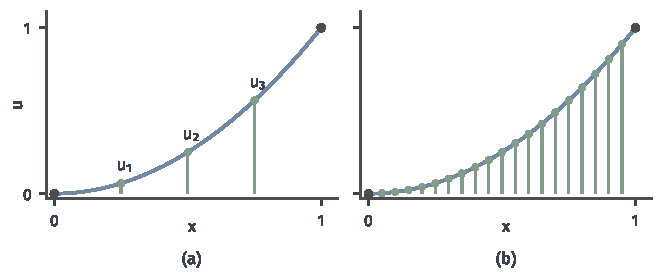
\includegraphics[width=112mm]{figures/05-optimization/08-functional-optimization/matplotlib/func-grid-vector/figure.pdf}
  \caption{函数$u(x)=x^2$的结点值。灰色点是被端点约束固定的值，绿色竖线是自由坐标。(a)$n=4$，自由坐标$u_1,u_2,u_3$。(b)$n=20$，自由坐标有$19$个。切得越细，向量越长，曲线的形状也记录得越完整。}
  \label{fig:func-grid-vector}
\end{BookInlineFigure}

用差商代替导数，用求和代替积分，式~\eqref{eq:func-energy}变成一个普通的多元函数。其中$u'^2$一项写成
\[
 \int_0^1\frac12u'(x)^2\,\mathrm{d}x\approx\sum_{i=0}^{n-1}\frac{\Delta}{2}\Bigl(\frac{u_{i+1}-u_i}{\Delta}\Bigr)^2
 =\frac{1}{2\Delta}\sum_{i=0}^{n-1}(u_{i+1}-u_i)^2.
\]
这是自由坐标的二次函数。取$n=2$，唯一的自由坐标是$u_1$。对$u^2$一项用梯形求积，得到一元二次函数
\[
 E_2(u_1)=u_1^2+(1-u_1)^2+\frac14u_1^2+\frac18.
\]
令导数$2u_1-2(1-u_1)+\frac12u_1$为零，解出$u_1=4/9\approx0.444$。这是用一个坐标对曲线中点高度的估计。

对应关系可以列成一张表，它只是起点，更多的对应要到后面几节才能建立。

\begin{BookInlineTable}
  \centering
  \caption{向量与函数的对应关系。}
  \label{tab:func-analogy}
  \begin{tabular}{ll}
    \toprule
    向量 $\bm{x}\in\mathbb{R}^n$ & 函数 $u$\\
    \midrule
    下标 $i$ & 位置 $x$\\
    坐标 $x_i$ & 取值 $u(x)$\\
    求和 $\sum_ix_iy_i$ & 积分 $\int u(x)v(x)\,\mathrm{d}x$\\
    目标函数 $f(\bm{x})$ & 目标泛函 $J(u)$\\
    线性约束的解集 & 固定边界值的函数集\\
    \bottomrule
  \end{tabular}
\end{BookInlineTable}

这个类比能直接告诉我们该问什么，却不能直接给出答案。$n$变大时维数没有上限，有限维里“维数固定”才成立的结论都要重新检查。

\paragraph{问题的写法}
有了具体例子，就可以写出一般形式。函数虽然被看成向量，写法上不加粗，可行集仍记作$\bm{C}$。

\begin{definition}[泛函优化问题]
\label{def:func-problem}
设$X$是实赋范空间，$\bm{C}\subseteq X$非空，$J:\bm{C}\to\mathbb{R}\cup\{+\infty\}$，且至少有一点取有限值。把输入函数、输出实数的$J$称为\term{目标泛函}（objective functional），问题
\begin{equation}
 \min_{u\in\bm{C}}J(u)
 \label{eq:func-problem}
\end{equation}
称为\term{泛函优化问题}（functional optimization problem）。记$J^\star=\inf_{u\in\bm{C}}J(u)$。若$u^\star\in\bm{C}$使$J(u^\star)=J^\star$，称$u^\star$为最优解。
\end{definition}

这里的\term{泛函}（functional）指定义在函数集合上、取值为数的映射。有限维问题只要写目标和约束，因为$\mathbb{R}^n$上的范数彼此等价，谈“附近”时不用说明用哪个范数。函数问题多出一项要写：空间$X$及其范数。它规定了三件事：哪些函数算候选，目标在哪里有限，两个函数怎样才算接近。

\paragraph{选择函数空间}
以$E$为例比较三个候选空间。若取$X=C^1[0,1]$，后面会看到极小化序列可能跑出这个空间；此外$E$用到的是导数的平方积分，它并不是$C^1$范数。若取$X=L^2(0,1)$，空间很大，但多数函数没有平方可积的导数，$E$只能取$+\infty$，端点值也没有意义，因为改变函数在一点的值不改变$L^2$中的元素。

合适的选择是让目标所用的量正好被范数控制，也就是取Sobolev空间
\begin{equation}
 H^1(0,1)=\bigl\{u\in L^2(0,1):u'\in L^2(0,1)\bigr\},\qquad
 \lVert u\rVert_{H^1}^2=\lVert u\rVert_2^2+\lVert u'\rVert_2^2.
 \label{eq:func-h1}
\end{equation}
其中$u'$是弱导数。$H^1(0,1)$是Hilbert空间，式~\eqref{eq:func-energy}的$E$恰好等于$\frac12\lVert u\rVert_{H^1}^2$。

下面要用到这个空间的三条性质。第一，每个$u\in H^1(0,1)$有连续代表，$u(y)-u(x)=\int_x^yu'(t)\,\mathrm{d}t$，所以端点值有意义。第二，点值受范数控制：
\begin{equation}
 \lvert u(y)\rvert\leq\sqrt2\,\lVert u\rVert_{H^1},\qquad y\in[0,1].
 \label{eq:func-point-bound}
\end{equation}
因此读取一点的值是$H^1(0,1)$上的连续线性泛函，在$L^2$中则不连续。第三，记端点为零的子空间为$H^1_0(0,1)$，其上有Poincaré不等式$\lVert v\rVert_2\leq\lVert v'\rVert_2$。这些结论的证明可参考\BookChapterRef{chap:sobolev-spaces}{卷四第21章“Sobolev空间”}。

\paragraph{允许怎样改变候选}
在$X=H^1(0,1)$中，端点条件~\eqref{eq:func-endpoints}给出可行集
\begin{equation}
 \bm{C}=\bigl\{u\in H^1(0,1):u(0)=0,\ u(1)=1\bigr\}.
 \label{eq:func-feasible}
\end{equation}
它不是线性子空间：两个可行函数的和在$x=1$处等于$2$。但两个可行函数的差在两端都为零。取$u_0(x)=x$，于是
\begin{equation}
 \bm{C}=u_0+\bm{V},\qquad \bm{V}=H^1_0(0,1).
 \label{eq:func-affine}
\end{equation}
这与线性方程组$\bm{A}\bm{x}=\bm{b}$的解集写成特解加零空间$\bm{x}_0+\operatorname{null}\bm{A}$完全相同。两个端点条件相当于两条线性约束，子空间$\bm{V}$只比$H^1(0,1)$少两个方向，但它仍是无限维的。

图~\ref{fig:func-feasible-directions}画了几个可行候选和它们与$u_0$的差。候选彼此差别很大，但(b)中所有的差都在两端归零。今后把这样的差称为扰动，记作$\eta$。求最优解时只能沿$\bm{V}$中的方向改变候选，这是第~\ref{sec:func-optimality}节最优性条件的出发点。

\begin{BookInlineFigure}
  \centering
  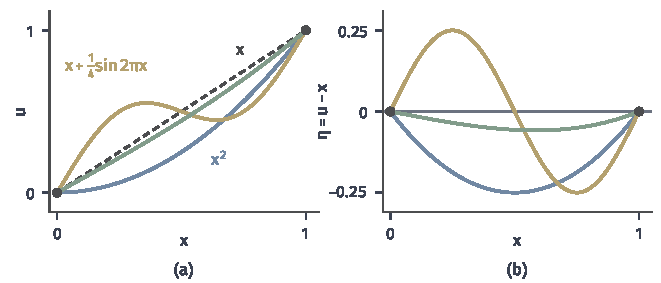
\includegraphics[width=112mm]{figures/05-optimization/08-functional-optimization/matplotlib/func-feasible-directions/figure.pdf}
  \caption{固定端点下的候选与扰动。(a)过$(0,0)$与$(1,1)$的候选：灰色虚线$u_0=x$、蓝色$x^2$、黄色$x+\frac14\sin2\pi x$，绿色是$\sinh x/\sinh1$。(b)同样颜色的三个差$\eta=u-x$，它们都在端点为零，属于方向子空间$\bm{V}=H^1_0(0,1)$。}
  \label{fig:func-feasible-directions}
\end{BookInlineFigure}

约束不同，允许的扰动也不同。若只固定$u(1)=1$而放开$u(0)$，扰动在$x=0$处可以取任意值，方向多了一个。若要求曲线处处不低于一个给定函数$\psi$，某些位置只能向上改动，能走的方向就依赖当前的候选。可行方向的这些差别，后面都会反映到最优性条件里。

\section{极小值的存在}
\label{sec:func-existence}

不解任何方程，怎样断定一个泛函优化问题有解？这件事比有限维更需要先做，因为后面的最优性条件都以“设$u^\star$是极小点”开头，极小点若不存在，由条件解出的东西就没有意义。

\paragraph{有限维的论证在哪里断开}
第~\ref{chap:optimization}章的论证是：取一个最小化序列，让它通过三关。序列要留得住，极限要合法，比较要能传到极限。在$\mathbb{R}^n$中，有界序列总有收敛子列，第一关由强制性和紧性解决。

无限维中这一步断开了。取$L^2(0,1)$中的函数$e_k(x)=\sqrt2\sin(k\pi x)$，$k=1,2,\ldots$。它们两两正交，长度都是$1$，于是
\[
 \lVert e_j-e_k\rVert_2=\sqrt2\qquad(j\neq k).
\]
这个序列在单位闭球内，任意两项的距离却始终是$\sqrt2$，没有Cauchy子列，也就没有范数收敛的子列。有界闭集不再紧。

\paragraph{换一种看极限的方式}
图~\ref{fig:func-weak-oscillation}(a)的$e_k$越摆越快，但摆动的正负会相互抵消。若固定一个函数$g$，用积分读取$\langle g,e_k\rangle=\int_0^1g\,e_k\,\mathrm{d}x$，(b)中的读数趋于零，而(a)中函数本身的长度不变。逐个读数都收敛到零，整个函数却没有在范数下靠近零。

\begin{BookInlineFigure}
  \centering
  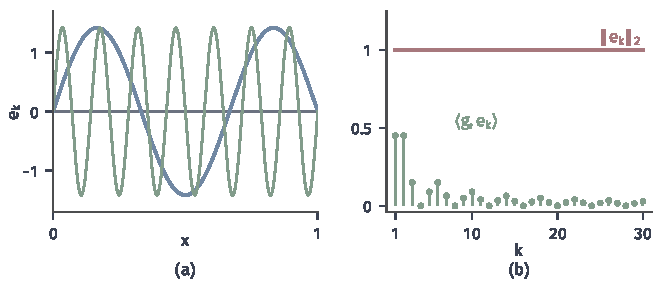
\includegraphics[width=112mm]{figures/05-optimization/08-functional-optimization/matplotlib/func-weak-oscillation/figure.pdf}
  \caption{弱收敛而范数不收敛。(a)$e_k=\sqrt2\sin(k\pi x)$，蓝色$k=3$，绿色$k=14$。(b)红线是$\lVert e_k\rVert_2=1$，绿色竖线是用$g=\mathbf{1}_{[0,1/2]}$读取的$\lvert\langle g,e_k\rangle\rvert$，它随$k$趋于零。}
  \label{fig:func-weak-oscillation}
\end{BookInlineFigure}

这种“每个连续读取都收敛”的收敛称为弱收敛。设$X$是赋范空间，$X^*$是它的对偶空间，即全体连续线性泛函。若对每个$\xi\in X^*$都有$\xi(u^{(k)})\to\xi(u)$，就说$u^{(k)}$弱收敛到$u$，记作$u^{(k)}\rightharpoonup u$。在Hilbert空间中，这就是对每个$g$都有$\langle g,u^{(k)}\rangle\to\langle g,u\rangle$。

弱收敛正好补上第一关。我们使用两条结论。若$X$是反射空间，则每个有界序列都有弱收敛的子列；Hilbert空间和$1<p<\infty$的$L^p$都是反射空间，$L^1$不是。若$u^{(k)}\rightharpoonup u$，则$\lVert u\rVert\leq\liminf_k\lVert u^{(k)}\rVert$，即弱极限的范数不会变大。证明可参考\BookChapterRef{chap:linear-functionals}{卷四第16章“线性泛函”}，后面要用的Riesz表示定理也在同一章。上面的$e_k$弱收敛到$0$，而$\lVert0\rVert_2=0<1$，不等号可以严格成立。

代价是后两关要跟着变。极限现在是弱极限，所以要求可行集对弱极限封闭，要求目标对弱极限不向上跳。

\begin{definition}[弱序列闭与弱序列下半连续]
\label{def:func-weak-lsc}
设$\bm{C}\subseteq X$。若$\bm{C}$中序列的每个弱极限仍在$\bm{C}$中，称$\bm{C}$\term{弱序列闭}（weakly sequentially closed）。设$J:\bm{C}\to\mathbb{R}\cup\{+\infty\}$，若对$\bm{C}$中每个弱收敛到$u\in\bm{C}$的序列都有
\begin{equation}
 J(u)\leq\liminf_{k\to\infty}J(u^{(k)}),
 \label{eq:func-weak-lsc}
\end{equation}
称$J$\term{弱序列下半连续}（weakly sequentially lower semicontinuous）。
\end{definition}

弱收敛比范数收敛容易发生，要对所有弱收敛序列成立的性质就更难满足。弱序列闭蕴含闭，反过来不成立；弱序列下半连续蕴含下半连续，反过来也不成立。

\paragraph{存在定理}
三关都有了新形式，图~\ref{fig:func-direct-gates}把它们排成一条链，并在下方列出有限维的对应要求。有限维中“有界”和“有收敛子列”由同一条性质负责，无限维中分成了两步：强制性给出有界，反射性给出弱子列。

\begin{BookInlineFigure}
  \centering
  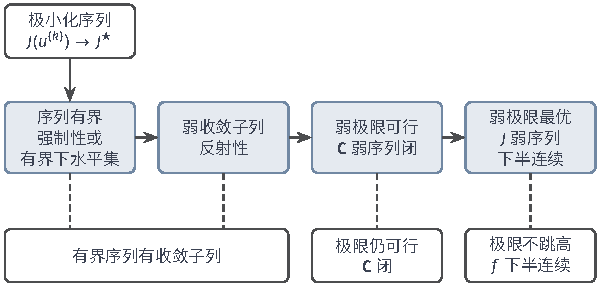
\includegraphics{figures/05-optimization/08-functional-optimization/tikz/func-direct-gates/figure.pdf}
  \caption{直接法的四步。上排蓝框是函数空间中的要求，每一步下方的白框是有限维的对应要求，有限维中有界序列必有收敛子列，所以前两步合成一个要求。}
  \label{fig:func-direct-gates}
\end{BookInlineFigure}

\begin{theorem}[直接法]
\label{thm:func-direct-method}
设$X$是实反射Banach空间，$\bm{C}\subseteq X$非空且弱序列闭，$J:\bm{C}\to\mathbb{R}\cup\{+\infty\}$弱序列下半连续。若存在实数$a$，使下水平集
\begin{equation}
 \bm{S}_a=\{u\in\bm{C}:J(u)\leq a\}
 \label{eq:func-sublevel}
\end{equation}
非空且有界，则$J^\star$是有限实数，且问题~\eqref{eq:func-problem}有最优解。
\end{theorem}

\begin{proof}
由$\bm{S}_a$非空，有$J^\star\leq a$。若$J^\star=a$，$\bm{S}_a$中的任一点已是最优解。下设$J^\star<a$，取$\bm{C}$中的序列$u^{(k)}$，使$J(u^{(k)})$递减到$J^\star$，并使各项都不超过$a$。这样的序列称为极小化序列，这里$J^\star$暂时可能是$-\infty$。

序列全在有界集$\bm{S}_a$中。$X$反射，所以有子列弱收敛到某个$u^\star\in X$，子列仍记作$u^{(k)}$。$\bm{C}$弱序列闭，所以$u^\star\in\bm{C}$。由弱序列下半连续性，
\[
 J(u^\star)\leq\liminf_{k\to\infty}J(u^{(k)})=J^\star.
\]
$J$不取$-\infty$，所以$J^\star$有限。又因$u^\star$可行，有$J(u^\star)\geq J^\star$，两式合起来得到$J(u^\star)=J^\star$。
\end{proof}

这种方法不写任何方程，直接对最小化序列取极限，称为\term{直接法}（direct method）。下水平集有界的最常见来源是强制性，即$\lVert u\rVert\to\infty$时$J(u)\to+\infty$。各条件的作用是：有界集把序列留住，反射性从中选出弱极限，弱序列闭保证弱极限合法，弱序列下半连续保证弱极限不比序列差。

\paragraph{怎样检查弱条件}
定义里的条件要对所有弱收敛序列验证，直接检查很困难。凸性把它们化成了容易检查的范数条件。先看可行集。

\begin{lemma}[闭凸集弱序列闭]
\label{lem:func-convex-weak-closed}
设$H$是Hilbert空间，$\bm{C}\subseteq H$是闭凸集。则$\bm{C}$弱序列闭。
\end{lemma}

\begin{proof}
设$u^{(k)}\in\bm{C}$，$u^{(k)}\rightharpoonup u$。令$p$为$u$到$\bm{C}$的最近点：到$\bm{C}$的距离的极小化序列，由平行四边形恒等式和凸性是Cauchy列，它的极限就是$p$。

任取$c\in\bm{C}$，$t\in(0,1]$，点$p+t(c-p)$在$\bm{C}$中，所以它到$u$的距离不小于$\lVert u-p\rVert_2$。展开平方，除以$t$，再令$t\to0$，得到
\[
 \langle u-p,\,c-p\rangle\leq0.
\]
取$c=u^{(k)}$，让$k\to\infty$。左端是固定向量$u-p$对$u^{(k)}-p$的读取，由弱收敛，得到
\[
 \lVert u-p\rVert^2=\langle u-p,\,u-p\rangle\leq0.
\]
所以$u=p\in\bm{C}$。
\end{proof}

几何上，证明说的是：若弱极限在$\bm{C}$之外，就有一个超平面把它和$\bm{C}$分开，而这个超平面对应的线性读取在弱收敛下是连续的，序列不可能跨过去。一般Banach空间中结论同样成立，称为Mazur定理，证明把最近点换成Hahn--Banach分离定理。

\begin{lemma}[凸与下半连续蕴含弱序列下半连续]
\label{lem:func-convex-weak-lsc}
设$\bm{C}$是Hilbert空间中的闭凸集，$J:\bm{C}\to\mathbb{R}\cup\{+\infty\}$是凸函数，且在范数下下半连续。则$J$弱序列下半连续。
\end{lemma}

\begin{proof}
对实数$a$，由$J$凸知$\bm{S}_a$是凸集，由下半连续和$\bm{C}$闭知$\bm{S}_a$是闭集，再由引理~\ref{lem:func-convex-weak-closed}，$\bm{S}_a$弱序列闭。

设$u^{(k)}\rightharpoonup u$，但$\liminf_kJ(u^{(k)})<J(u)$。取实数$a$严格介于两者之间，则有子列落在$\bm{S}_a$中。它的弱极限$u$也在$\bm{S}_a$中，即$J(u)\leq a$，与$a<J(u)$矛盾。
\end{proof}

回到式~\eqref{eq:func-energy}。可行集~\eqref{eq:func-feasible}是由两个连续线性条件给出的闭仿射集，是闭凸集；由式~\eqref{eq:func-point-bound}，端点读取在$H^1$中连续。$E=\frac12\lVert u\rVert_{H^1}^2$是凸的连续函数，下水平集都有界。定理~\ref{thm:func-direct-method}的条件全部满足，所以$E$的极小点存在。

\paragraph{积分目标的存在定理}
下面的结论把上述检查做成一个可以直接使用的形式。它把密度分成导数部分和函数值部分，两部分起的作用不同。

\begin{theorem}[可分离密度的存在性]
\label{thm:func-tonelli}
设$G:\mathbb{R}\to\mathbb{R}$是凸的连续函数，并存在$c>0$和$d\geq0$使$G(p)\geq cp^2-d$。设$V:[0,1]\times\mathbb{R}\to\mathbb{R}$连续且下有界。对给定的实数$\alpha,\beta$，在
\begin{equation}
 \bm{C}=\bigl\{u\in H^1(0,1):u(0)=\alpha,\ u(1)=\beta\bigr\}
 \label{eq:func-separable-feasible}
\end{equation}
上，目标
\begin{equation}
 J(u)=\int_0^1\Bigl(G\bigl(u'(x)\bigr)+V\bigl(x,u(x)\bigr)\Bigr)\,\mathrm{d}x
 \label{eq:func-separable}
\end{equation}
有极小点。
\end{theorem}

\begin{proof}
\emph{有界下水平集。}线性函数$u_0$过两个端点，$J(u_0)$有限；取$a=J(u_0)$。设$J(u)\leq a$，$V\geq-d'$，由增长条件，
\[
 c\lVert u'\rVert_2^2\leq a+d+d'.
\]
$u-u_0\in H^1_0(0,1)$，由Poincaré不等式，$\lVert u-u_0\rVert_2\leq\lVert u'-u_0'\rVert_2$。所以$\bm{S}_a$在$H^1$中有界。

\emph{可行集。}$\bm{C}$是闭仿射集，由引理~\ref{lem:func-convex-weak-closed}，它弱序列闭。

\emph{弱序列下半连续。}设$u^{(k)}\rightharpoonup u$于$H^1$，取子列使$J(u^{(k)})$趋于下极限，不妨设下极限有限。弱收敛序列有界，再由连续代表的等式和Cauchy--Schwarz不等式，
\[
 \lvert u^{(k)}(x)-u^{(k)}(y)\rvert\leq\lvert x-y\rvert^{1/2}\lVert u^{(k)\prime}\rVert_2.
\]
所以$u^{(k)}$一致有界且等度连续。由Arzelà--Ascoli定理，再取子列，它在$[0,1]$上一致收敛，极限必为$u$。$V$在紧集上一致连续，于是
\[
 \int_0^1V(x,u^{(k)})\,\mathrm{d}x\to\int_0^1V(x,u)\,\mathrm{d}x.
\]

对每个$g\in L^2$，$v\mapsto\int_0^1gv'\,\mathrm{d}x$是$H^1$上的连续线性泛函，所以$u^{(k)\prime}\rightharpoonup u'$于$L^2$。泛函$w\mapsto\int_0^1G(w)\,\mathrm{d}x$在$L^2$上是凸的。它也下半连续：范数收敛序列有几乎处处收敛的子列，$G+d\geq0$，对其用Fatou引理即可。由引理~\ref{lem:func-convex-weak-lsc}，
\[
 \int_0^1G(u')\,\mathrm{d}x\leq\liminf_{k\to\infty}\int_0^1G(u^{(k)\prime})\,\mathrm{d}x.
\]
两部分相加即得式~\eqref{eq:func-weak-lsc}，再由定理~\ref{thm:func-direct-method}得到结论。
\end{proof}

证明展示了分工。函数值$u^{(k)}$因为一维的紧嵌入而一致收敛，所以$V$不需要任何凸性。导数$u^{(k)\prime}$只有弱收敛，所以$G$必须对$p$是凸的。$E$的$G=\frac12p^2$，$V=\frac12s^2$，满足定理。

\paragraph{第一关失败：序列没有界，或者没有弱极限}
下面逐条去掉条件。第一个例子去掉强制性。考虑区间$[-1,1]$上的目标
\[
 J(u)=\int_{-1}^1x^2u'(x)^2\,\mathrm{d}x,\qquad u(-1)=-1,\ u(1)=1.
\]
权函数$x^2$在原点为零，那里的导数几乎不被惩罚。取图~\ref{fig:func-fail-bounded}(a)的折线$u^{(k)}(x)=\max\{-1,\min\{1,kx\}\}$，导数只在$\lvert x\rvert<1/k$上非零，等于$k$。代入得到
\[
 J(u^{(k)})=\int_{-1/k}^{1/k}x^2k^2\,\mathrm{d}x=\frac{2}{3k}\to0.
\]

所以$J^\star=0$。若有$u\in H^1(-1,1)$使$J(u)=0$，则$u'=0$几乎处处，$u$是常数，这与两端的值$-1,1$矛盾，极小点不存在。此时导数的长度$\lVert u^{(k)\prime}\rVert_2^2=2k$趋于无穷，序列在$H^1$中无界，$J$不强制。序列想要趋向的跳跃函数也不在$H^1$中。

\begin{BookInlineFigure}
  \centering
  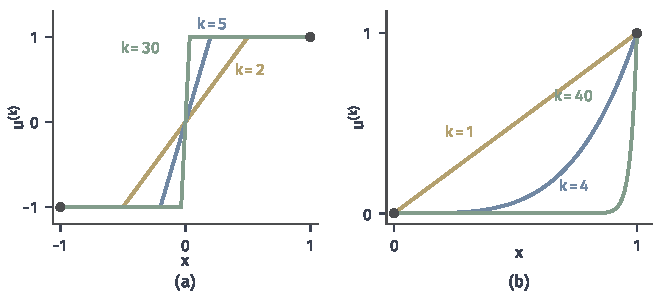
\includegraphics[width=112mm]{figures/05-optimization/08-functional-optimization/matplotlib/func-fail-bounded/figure.pdf}
  \caption{第一关的两种失败，灰点是固定端点。(a)$\int_{-1}^1x^2u'^2\,\mathrm{d}x$的极小化序列$u^{(k)}=\max\{-1,\min\{1,kx\}\}$，目标值$2/(3k)$趋于零，导数的长度趋于无穷。(b)$\int_0^1(\lvert u'\rvert+u^2)\,\mathrm{d}x$的极小化序列$u^{(k)}=x^k$，$W^{1,1}$范数有界，所有质量向$x=1$处的跳跃集中。}
  \label{fig:func-fail-bounded}
\end{BookInlineFigure}

第二个例子去掉反射性。在$W^{1,1}(0,1)$上取端点条件$u(0)=0$、$u(1)=1$，目标
\[
 J(u)=\int_0^1\bigl(\lvert u'(x)\rvert+u(x)^2\bigr)\,\mathrm{d}x.
\]
曲线从$0$升到$1$，导数绝对值的积分不小于总上升量：
\[
 \int_0^1\lvert u'\rvert\,\mathrm{d}x\geq\lvert u(1)-u(0)\rvert=1.
\]
所以$J\geq1$。取图~\ref{fig:func-fail-bounded}(b)的$u^{(k)}=x^k$，它单调上升，所以
\[
 J(u^{(k)})=1+\frac{1}{2k+1}\to1.
\]

因此$J^\star=1$。若$J(u)=1$，则$\int_0^1u^2\,\mathrm{d}x=0$，$u$恒为零，与$u(1)=1$矛盾，极小点不存在。这次序列有界，它的$W^{1,1}$范数满足
\[
 \lVert u^{(k)}\rVert_1+\lVert u^{(k)\prime}\rVert_1\leq2.
\]
但它没有弱收敛子列。若有，弱极限几乎处处等于序列的逐点极限$0$，而端点读取在$W^{1,1}$中连续，弱极限在$x=1$处又应等于$1$。把平方积分的$\lvert u'\rvert^2$换成$\lvert u'\rvert$，反射性就失去了，定理~\ref{thm:func-tonelli}中$cp^2$的增长条件正是在防止这种情况。

\paragraph{第二关失败：弱极限不可行}
闭集未必弱序列闭。取$\bm{C}$为$L^2(0,1)$中的单位球面，目标$J(u)=\int_0^1x\,u(x)^2\,\mathrm{d}x$。这相当于分配总量为$1$的质量，放在$x$处的代价是$x$，质量当然想挤到原点。取$u^{(k)}=\sqrt{k}\,\mathbf{1}_{[0,1/k]}$，见图~\ref{fig:func-fail-sphere}，得到
\[
 \lVert u^{(k)}\rVert_2=1,\qquad J(u^{(k)})=k\int_0^{1/k}x\,\mathrm{d}x=\frac{1}{2k}\to0.
\]

\begin{BookInlineFigure}
  \centering
  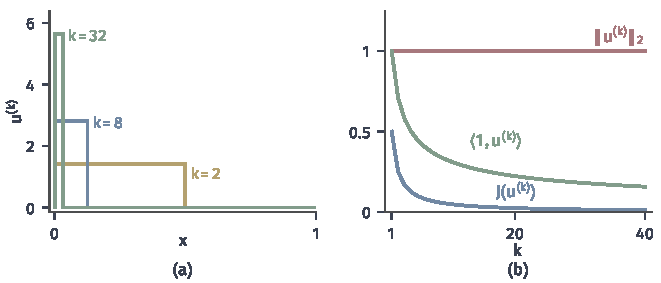
\includegraphics[width=112mm]{figures/05-optimization/08-functional-optimization/matplotlib/func-fail-sphere/figure.pdf}
  \caption{第二关的失败：单位球面不弱序列闭。(a)$u^{(k)}=\sqrt{k}\,\mathbf{1}_{[0,1/k]}$越来越高、越来越窄。(b)红线是不变的长度，绿线是读取$\langle1,u^{(k)}\rangle=k^{-1/2}$，蓝线是目标值$1/(2k)$。}
  \label{fig:func-fail-sphere}
\end{BookInlineFigure}

$J(u)=0$要求$u=0$几乎处处，但零函数不在球面上，所以极小点不存在。对任意$g\in L^2$，由Cauchy--Schwarz不等式，
\[
 \lvert\langle g,u^{(k)}\rangle\rvert\leq\lVert g\rVert_{L^2(0,1/k)}\to0.
\]
所以$u^{(k)}\rightharpoonup0$。球面上的序列弱收敛到球心，弱极限离开了可行集。在有限维中球面是紧集，这个现象不会发生。把可行集放大成单位闭球，它是闭凸集，极小点$u=0$立即存在。

\paragraph{第三关失败：弱极限比序列差}
最后去掉对导数的凸性。在$H^1(0,1)$上考虑
\begin{equation}
 J(u)=\int_0^1\Bigl(\bigl(u'(x)^2-1\bigr)^2+u(x)^2\Bigr)\,\mathrm{d}x,\qquad u(0)=u(1)=0,
 \label{eq:func-bolza}
\end{equation}
其中$u'\notin L^4$时$J$取$+\infty$。第一项希望斜率是$\pm1$，第二项希望$u$接近零。取图~\ref{fig:func-bolza-zigzag}(a)的锯齿$z_k$：$k$个相同的齿，斜率$\pm1$，高度$1/(2k)$。第一项为零，第二项每个齿贡献$\frac{2}{3}(2k)^{-3}$，总计
\[
 J(z_k)=k\cdot\frac23\cdot\frac{1}{8k^3}=\frac{1}{12k^2}\to0.
\]

\begin{BookInlineFigure}
  \centering
  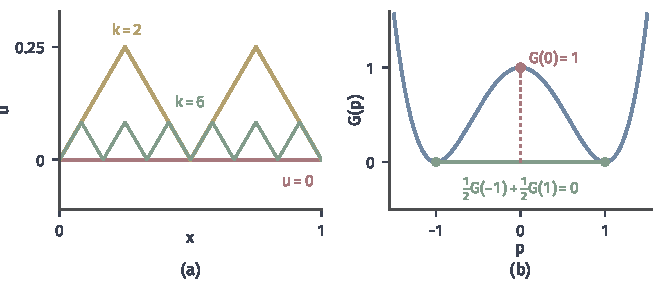
\includegraphics[width=112mm]{figures/05-optimization/08-functional-optimization/matplotlib/func-bolza-zigzag/figure.pdf}
  \caption{第三关的失败。(a)目标~\eqref{eq:func-bolza}的锯齿极小化序列，黄色$k=2$，绿色$k=6$，红线是弱极限$u=0$。(b)导数部分的密度$G(p)=(p^2-1)^2$：斜率$\pm1$各占一半时，平均代价是绿线上的$0$，而平均斜率$0$自身的代价是红点$1$。}
  \label{fig:func-bolza-zigzag}
\end{BookInlineFigure}

所以$J^\star=0$。$J(u)=0$要求$u=0$，同时要求$\lvert u'\rvert=1$几乎处处，二者矛盾，极小点不存在。序列在$H^1$中有界，并且$z_k\rightharpoonup0$，弱极限$0$是可行的，但$J(0)=1$。弱极限比序列差了整整一个单位，式~\eqref{eq:func-weak-lsc}不成立。

机制在图~\ref{fig:func-bolza-zigzag}(b)。弱收敛只记住了斜率的局部平均，而锯齿的平均斜率是$0$。$G$在$\pm1$处为零，而在两者的平均$0$处等于$1$，这就是$G$非凸。若$G$是凸的，Jensen不等式给出“平均的代价不超过代价的平均”，弱极限就不会变差。

\paragraph{驻定不能代替存在}
还有一种常见的想法：写出令导数为零的方程，解出来就是答案。下面的例子说明，这样做既不能证明解存在，得到的候选也未必是解。在$\bm{V}=H^1_0(0,1)$上取实数$\rho$，考虑
\begin{equation}
 J_\rho(u)=\int_0^1\Bigl(\frac12u'(x)^2-\frac{\rho}{2}u(x)^2\Bigr)\,\mathrm{d}x.
 \label{eq:func-rho}
\end{equation}
沿任何一条过原点的直线都有$J_\rho(t\eta)=t^2J_\rho(\eta)$，这是$t$的一元二次函数，在$t=0$处导数为零。所以$u=0$沿每个方向都是平的，它满足任何合理的驻定条件。

取方向$\eta(x)=\sin\pi x$。由$\int_0^1\eta'^2\,\mathrm{d}x=\pi^2/2$，$\int_0^1\eta^2\,\mathrm{d}x=1/2$，得到
\[
 J_\rho(t\sin\pi x)=\frac{t^2}{4}(\pi^2-\rho).
\]
图~\ref{fig:func-stationary-no-min}画了三种情形。$\rho>\pi^2$时，沿这个方向目标趋于$-\infty$，$J_\rho^\star=-\infty$，极小点不存在，而$u=0$仍然驻定。

\begin{BookInlineFigure}
  \centering
  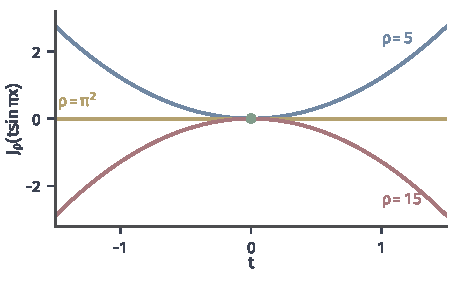
\includegraphics[width=78mm]{figures/05-optimization/08-functional-optimization/matplotlib/func-stationary-no-min/figure.pdf}
  \caption{目标~\eqref{eq:func-rho}沿$t\sin\pi x$的取值。绿点$t=0$在三种情形下都驻定。$\rho=5$时是开口向上的抛物线，$\rho=\pi^2$时恒为零，$\rho=15$时向下，目标无下界。}
  \label{fig:func-stationary-no-min}
\end{BookInlineFigure}

这个$J_\rho$对每个$\rho$都弱序列下半连续：$\int u'^2$部分是凸的，$\int u^2$部分在弱收敛下连续。失败的只是下水平集的有界性。“若极小点存在，则它满足驻定方程”是一个条件命题，它的前提要靠本节的论证另行建立。

\section{泛函的微分}
\label{sec:func-differential}

有限维中，一点处的梯度告诉我们目标沿每个方向的一阶变化。这就需要回答：对泛函，同样的事情怎样表述？方向上的变化率总可以先算，它能否合成一个线性近似，线性近似又能否写成一个梯度，这是三个不同的问题。

\subsection{方向微分与线性近似}
\label{sec:func-directional}

\paragraph{沿一条直线看}
给定候选$u$和扰动$\eta$，让实数$t$控制扰动的大小。整条曲线沿“方向”$\eta$移动，目标变成一元函数
\begin{equation}
 \phi(t)=J(u+t\eta).
 \label{eq:func-phi}
\end{equation}
这是最重要的一步化归：一元函数我们已经会求导。

下面用式~\eqref{eq:func-energy}的$E$计算一次。取$u(x)=x$，$\eta(x)=x(1-x)$，它们满足$\eta(0)=\eta(1)=0$，所以$x+t\eta$对每个$t$都可行。导数是$(x+t\eta)'=1+t(1-2x)$，代入后按$t$的幂次展开，需要三个积分：
\[
 \int_0^1(1-2x)\,\mathrm{d}x=0,\qquad
 \int_0^1(1-2x)^2\,\mathrm{d}x=\frac13,\qquad
 \int_0^1x\cdot x(1-x)\,\mathrm{d}x=\frac1{12}.
\]
再加上$\int_0^1x^2(1-x)^2\,\mathrm{d}x=\frac1{30}$和$E(x)=\frac23$，得到
\begin{equation}
 \phi(t)=\frac23+\frac{t}{12}+\frac{11}{60}t^2.
 \label{eq:func-phi-example}
\end{equation}
所以$\phi'(0)=1/12$。图~\ref{fig:func-direction-family}的(a)是这一族曲线，(b)是$\phi$及其切线。注意这里求导的变量是$t$，不是$x$：$u'(x)$描述一条固定曲线的陡峭程度，$\phi'(0)$描述整条曲线改动时目标的响应。

\begin{BookInlineFigure}
  \centering
  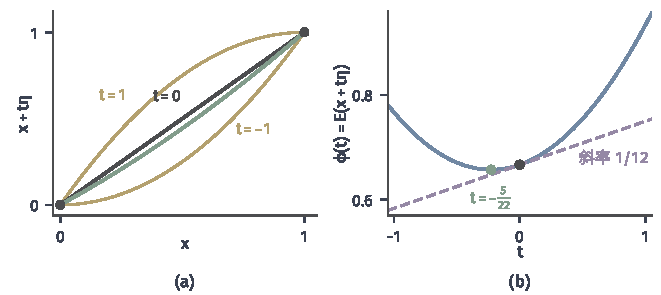
\includegraphics[width=112mm]{figures/05-optimization/08-functional-optimization/matplotlib/func-direction-family/figure.pdf}
  \caption{沿一个方向改动整条曲线。(a)$u=x$（深灰）和$\eta=x(1-x)$给出的曲线族$x+t\eta$，黄色$t=\pm1$，绿色$t=-5/22$，端点不动。(b)$\phi(t)=E(x+t\eta)$，紫色虚线是$t=0$处的切线，斜率$1/12$；绿点是这条直线上的最小点$t=-5/22$。}
  \label{fig:func-direction-family}
\end{BookInlineFigure}

$\phi$在$t=-5/22$处最小，说明沿这个方向还能下降，$x$不是极小点。这个判断只用了一元微积分。

\begin{definition}[方向导数]
\label{def:func-directional}
设$X$是实赋范空间，$J(u)$有限，$\eta\in X$，且$t>0$充分小时$J(u+t\eta)$有限。若极限
\begin{equation}
 J'(u;\eta)=\lim_{t\downarrow0}\frac{J(u+t\eta)-J(u)}{t}
 \label{eq:func-directional}
\end{equation}
存在且有限，称它为$J$在$u$处沿$\eta$的\term{方向导数}（directional derivative）。
\end{definition}

定义只取$t\downarrow0$的单侧极限，因为有约束时常常只能朝一侧走。方向导数只回答一条直线上的问题，把所有方向的答案放在一起，未必是线性函数。在$L^2(0,1)$上取$J(u)=\int_0^1\lvert u\rvert\,\mathrm{d}x$，由齐次性直接得到$J'(0;\eta)=\int_0^1\lvert\eta\rvert\,\mathrm{d}x$。它对$\eta$不可加，$J'(0;\eta)+J'(0;-\eta)$也不为零。这与$\lvert x\rvert$在原点的尖角相同。

\paragraph{线性且连续：Gâteaux微分}
有限维中，光滑函数的方向导数是$\nabla f(\bm{x})^\top\bm{d}$，对$\bm{d}$线性。线性是我们想要的结构，无限维中还要多要求一件事：连续。有限维的线性函数自动连续，无限维的线性泛函不然。

\begin{definition}[Gâteaux微分]
\label{def:func-gateaux}
若$J'(u;\eta)$对每个$\eta\in X$存在，且$\eta\mapsto J'(u;\eta)$是$X$上的连续线性泛函，称$J$在$u$处\term{Gâteaux可微}（Gâteaux differentiable），称这个泛函为$J$在$u$处的\term{Gâteaux微分}（Gâteaux derivative），记作$DJ(u)\in X^*$，即
\begin{equation}
 DJ(u)[\eta]=J'(u;\eta).
 \label{eq:func-gateaux}
\end{equation}
\end{definition}

线性中已经包含$J'(u;-\eta)=-J'(u;\eta)$，所以这时$t\to0$的双侧极限也存在。Gâteaux微分还是逐方向定义的：对每个固定的$\eta$，$t$足够小时余项才小，“足够小”的程度可以随方向变化。

\paragraph{一致的余项：Fréchet微分}
真正的线性近似要求：只要扰动在范数下小，余项就比范数小，不管扰动沿哪个方向。

\begin{definition}[Fréchet微分]
\label{def:func-frechet}
设$J$在$u$的某邻域内有限。若存在$\xi\in X^*$使
\begin{equation}
 \lim_{\lVert\eta\rVert\to0}\frac{\lvert J(u+\eta)-J(u)-\xi(\eta)\rvert}{\lVert\eta\rVert}=0,
 \label{eq:func-frechet}
\end{equation}
称$J$在$u$处\term{Fréchet可微}（Fréchet differentiable），$\xi$称为Fréchet微分。
\end{definition}

两个定义的差别只在极限的取法。Gâteaux微分固定形状，只缩小幅度；Fréchet微分允许形状和幅度同时变化。无限维中形状可以无穷多，这个差别才变得实质。

\paragraph{一个Gâteaux可微而非Fréchet可微的泛函}
下面的例子说明，这个差别由范数决定。考虑
\begin{equation}
 S(u)=\int_0^1\sin\bigl(u(x)\bigr)\,\mathrm{d}x.
 \label{eq:func-sin}
\end{equation}
先在$X=L^1(0,1)$的$u=0$处计算方向导数。差商的被积函数$\sin(t\eta)/t$逐点趋于$\eta$，并被可积函数$\lvert\eta\rvert$控制，由控制收敛定理，
\[
 S'(0;\eta)=\int_0^1\eta(x)\,\mathrm{d}x.
\]
它线性，并且不超过$\lVert\eta\rVert_1$，所以$S$在$0$处Gâteaux可微。

再测试余项。取图~\ref{fig:func-spike-frechet}(a)的尖峰$\eta_k=\pi\mathbf{1}_{[0,1/k]}$，幅度始终是$\pi$，宽度趋于零。余项为
\[
 S(\eta_k)-S(0)-\int_0^1\eta_k\,\mathrm{d}x=\frac1k\bigl(\sin\pi-\pi\bigr)=-\frac{\pi}{k}.
\]
而$\lVert\eta_k\rVert_1=\pi/k$，比值的绝对值恒等于$1$，不趋于零。所以$S$在$L^1$中不是Fréchet可微的。

\begin{BookInlineFigure}
  \centering
  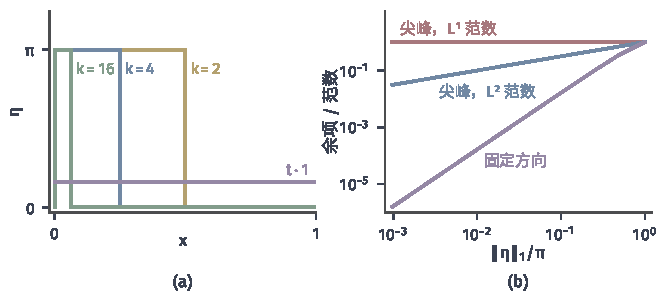
\includegraphics[width=112mm]{figures/05-optimization/08-functional-optimization/matplotlib/func-spike-frechet/figure.pdf}
  \caption{同一泛函$S(u)=\int_0^1\sin u\,\mathrm{d}x$在$u=0$处的余项。(a)尖峰扰动$\pi\mathbf{1}_{[0,1/k]}$（$k=2,4,16$）与固定方向的缩小$t\cdot1$（紫色）。(b)余项除以范数：尖峰在$L^1$范数下恒为$1$（红），在$L^2$范数下按$k^{-1/2}$衰减（蓝）；固定方向$t\cdot1$按$t^2$衰减（紫）。}
  \label{fig:func-spike-frechet}
\end{BookInlineFigure}

换成$X=L^2(0,1)$，同一个尖峰的范数是$\lVert\eta_k\rVert_2=\pi k^{-1/2}$，比$L^1$范数大得多，比值变成$k^{-1/2}\to0$。这不是巧合。由Taylor公式，逐点有
\[
 \lvert\sin(u+\eta)-\sin u-\eta\cos u\rvert\leq\frac12\eta^2.
\]
两边积分，得到
\[
 \Bigl\lvert S(u+\eta)-S(u)-\int_0^1\eta\cos u\,\mathrm{d}x\Bigr\rvert\leq\frac12\lVert\eta\rVert_2^2.
\]
所以$S$在$L^2$中处处Fréchet可微。在$L^1$中，窄而高的尖峰范数很小，函数值的改动却不小；$L^2$范数对尖峰更敏感，把它们排除在“小扰动”之外。讨论可微性时必须说清范数。

\paragraph{两种微分的关系}
下面的定理说明，Fréchet可微更强，以及在什么条件下两者相同。

\begin{theorem}[Gâteaux与Fréchet]
\label{thm:func-gateaux-frechet}
设$J$在$u$的某邻域内有限。
\begin{enumerate}
 \item 若$J$在$u$处Fréchet可微，则$J$在$u$处Gâteaux可微，且$DJ(u)=\xi$。
 \item 若$J$在$u$的邻域内Gâteaux可微，且映射$v\mapsto DJ(v)$在$u$处从$X$到$X^*$连续，则$J$在$u$处Fréchet可微。
\end{enumerate}
\end{theorem}

\begin{proof}
(1)固定$\eta\neq0$，在式~\eqref{eq:func-frechet}中用$t\eta$代替$\eta$，$t\downarrow0$时$\lVert t\eta\rVert\to0$。两边除以$t$，得到差商趋于$\xi(\eta)$。

(2)取$\lVert\eta\rVert$足够小，使线段$u+t\eta$（$t\in[0,1]$）落在邻域内。$\phi(t)=J(u+t\eta)$在$[0,1]$上可导，$\phi'(t)=DJ(u+t\eta)[\eta]$。由Lagrange中值定理，存在$\theta\in(0,1)$，使
\[
 J(u+\eta)-J(u)=DJ(u+\theta\eta)[\eta].
\]
两边减去$DJ(u)[\eta]$，再用对偶范数的定义，得到
\[
 \bigl\lvert J(u+\eta)-J(u)-DJ(u)[\eta]\bigr\rvert\leq\lVert DJ(u+\theta\eta)-DJ(u)\rVert\,\lVert\eta\rVert.
\]
由连续性，$\lVert\eta\rVert\to0$时右端的第一个因子趋于零。
\end{proof}

这解释了$S$在$L^1$中的情形：$DS(v)$是乘以$\cos v$的积分，$L^1$范数很小的尖峰可以让$\cos v$在一小段上改变一个固定的量，所以微分在$X^*=L^\infty$中不连续，第二条的条件不满足。

三个层次可以列表比较。

\begin{BookInlineTable}
  \centering
  \caption{一阶信息的三个层次。}
  \label{tab:func-derivative-levels}
  \begin{tabular}{lll}
    \toprule
    层次 & 要求 & 不满足下一层的例子\\
    \midrule
    方向导数 & 每条直线上有导数 & $\int_0^1\lvert u\rvert\,\mathrm{d}x$ 在 $u=0$\\
    Gâteaux微分 & 上述导数线性连续 & $\int_0^1\sin u\,\mathrm{d}x$ 在 $L^1$\\
    Fréchet微分 & 余项对方向一致 & ---\\
    \bottomrule
  \end{tabular}
\end{BookInlineTable}

\paragraph{能量的展开}
回到$E$。对$u,\eta\in H^1(0,1)$，把平方展开，不做任何近似：
\begin{equation}
 E(u+\eta)=E(u)+\int_0^1\bigl(u'\eta'+u\eta\bigr)\,\mathrm{d}x+\frac12\lVert\eta\rVert_{H^1}^2.
 \label{eq:func-energy-expansion}
\end{equation}
中间一项是$\eta$的线性泛函。由Cauchy--Schwarz不等式，它的绝对值不超过$\lVert u\rVert_{H^1}\lVert\eta\rVert_{H^1}$，所以连续。余项是$\frac12\lVert\eta\rVert_{H^1}^2$，比$\lVert\eta\rVert_{H^1}$高一阶。因此$E$在$H^1$中处处Fréchet可微，
\begin{equation}
 DE(u)[\eta]=\int_0^1\bigl(u'\eta'+u\eta\bigr)\,\mathrm{d}x.
 \label{eq:func-energy-derivative}
\end{equation}
取$u=x$，$\eta=x(1-x)$，右端是$\int_0^1(1-2x)\,\mathrm{d}x+\frac1{12}=\frac1{12}$，与式~\eqref{eq:func-phi-example}一致。长度目标也可以同样处理：$G(p)=\sqrt{1+p^2}$满足$0<G''\leq1$，由Taylor公式，余项不超过$\frac12\lVert\eta'\rVert_2^2$，所以$\ell$在$H^1$中Fréchet可微。

\subsection{Hilbert梯度}
\label{sec:func-hilbert-gradient}

微分$DJ(u)$是一个把方向读成数的线性泛函，它是“行向量”。梯度下降需要的却是一个能和候选相加的“列向量”。本小节要回答的问题是：怎样把微分转成梯度？答案取决于内积。

\paragraph{有限维中内积就已经起作用}
把向量和方向配对的是微分$Df(\bm{x})[\bm{d}]=\nabla f(\bm{x})^\top\bm{d}$，这里的$\nabla f$其实默认了欧氏内积。换一个内积，由对称正定矩阵$\bm{M}$给出：
\[
 \langle\bm{x},\bm{y}\rangle_{\bm{M}}=\bm{x}^\top\bm{M}\bm{y}.
\]
这时梯度应当是满足下式的向量$\bm{g}$，内积下读出的就是同一个微分：
\[
 \bm{g}^\top\bm{M}\bm{d}=\nabla f(\bm{x})^\top\bm{d}\qquad\text{对每个}\ \bm{d}.
\]
解出来就是
\begin{equation}
 \bm{g}=\bm{M}^{-1}\nabla f(\bm{x}).
 \label{eq:func-metric-gradient}
\end{equation}

用第~\ref{chap:smooth-foundations}章的例子$f(\bm{x})=\frac12(x_1^2+9x_2^2)$看，在$\bm{x}=(9,1)$处，$\nabla f=(9,9)$。取$\bm{M}=\operatorname{diag}(1,9)$，它是这个目标的Hessian，代入式~\eqref{eq:func-metric-gradient}，
\[
 \bm{g}=(9,1).
\]
图~\ref{fig:func-metric-gradient}中，黄色箭头是欧氏梯度方向的一步，绿色箭头沿$-\bm{g}$，一步直达原点。同一个微分，在两个内积下给出两个不同的梯度。“最速下降方向”依赖怎样度量步长的长度。

\begin{BookInlineFigure}
  \centering
  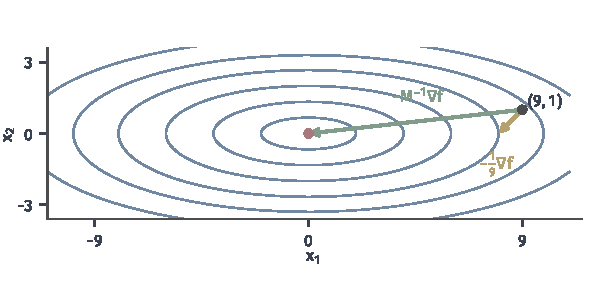
\includegraphics[width=100mm]{figures/05-optimization/08-functional-optimization/matplotlib/func-metric-gradient/figure.pdf}
  \caption{同一个微分在两个内积下的梯度。蓝色为$f=\frac12(x_1^2+9x_2^2)$的等高线，出发点$(9,1)$。黄色箭头是步长$1/9$的欧氏负梯度步，绿色箭头是$\bm{M}=\operatorname{diag}(1,9)$内积下步长$1$的负梯度步，终点是最优解（红点）。}
  \label{fig:func-metric-gradient}
\end{BookInlineFigure}

\paragraph{函数空间中的梯度}
有限维中$\bm{M}$可逆，这个转换永远可以做。在Hilbert空间中，转换由Riesz表示定理完成：$H$上的每个连续线性泛函$\xi$，都存在唯一的$w\in H$，使$\xi(\eta)=\langle w,\eta\rangle_H$对所有$\eta\in H$成立。

\begin{definition}[Hilbert梯度]
\label{def:func-hilbert-gradient}
设$H$是实Hilbert空间，$J$在$u$处沿$H$的方向Gâteaux可微。称满足
\begin{equation}
 DJ(u)[\eta]=\bigl\langle\nabla_HJ(u),\eta\bigr\rangle_H\qquad(\eta\in H)
 \label{eq:func-hilbert-gradient}
\end{equation}
的唯一元素$\nabla_HJ(u)\in H$为$J$在$u$处的\term{Hilbert梯度}（Hilbert gradient）。
\end{definition}

由Cauchy--Schwarz不等式，在$\lVert\eta\rVert_H=1$的方向中，$DJ(u)[\eta]$在$\eta$平行于$\nabla_HJ(u)$时最大，所以它确实是“上升最快的方向”，只是这里的“单位长度”用$H$的范数计量。

\paragraph{同一个微分的三个梯度}
下面算一个具体例子。对$E$在$u=x$处，方向取$\bm{V}=H^1_0(0,1)$。由式~\eqref{eq:func-energy-derivative}和$\int_0^1\eta'\,\mathrm{d}x=\eta(1)-\eta(0)=0$，得到
\begin{equation}
 DE(x)[\eta]=\int_0^1x\,\eta(x)\,\mathrm{d}x.
 \label{eq:func-de-at-x}
\end{equation}
这一个线性泛函，用三种内积表示。

第一种是$L^2$内积。式~\eqref{eq:func-de-at-x}已经写成了$\langle x,\eta\rangle_2$，所以$L^2$梯度是
\[
 w_1(x)=x.
\]
第二种内积只用导数：
\[
 \langle v,\eta\rangle_{\bm{V}}=\int_0^1v'\eta'\,\mathrm{d}x.
\]
由Poincaré不等式它是$\bm{V}$上的内积，$\bm{V}$在其下完备。要找$w_2\in\bm{V}$，使它在这个内积下读出式~\eqref{eq:func-de-at-x}。分部积分，边界项因$\eta$在端点为零而消失，问题化成$-w_2''=x$，$w_2(0)=w_2(1)=0$。解得
\[
 w_2(x)=\frac{x-x^3}{6}.
\]
第三种是$H^1$内积$\int_0^1(v'\eta'+v\eta)\,\mathrm{d}x$。同样分部积分，问题化成$-w_3''+w_3=x$，$w_3(0)=w_3(1)=0$。解得
\[
 w_3(x)=x-\frac{\sinh x}{\sinh1}.
\]

三个函数画在图~\ref{fig:func-three-gradients}中，形状和大小都不同，但它们表示同一个微分。用$\eta=x(1-x)$检验，三种内积给出的都是$1/12$。例如第二种：
\[
 \int_0^1\frac{1-3x^2}{6}(1-2x)\,\mathrm{d}x=\frac1{12}.
\]

\begin{BookInlineFigure}
  \centering
  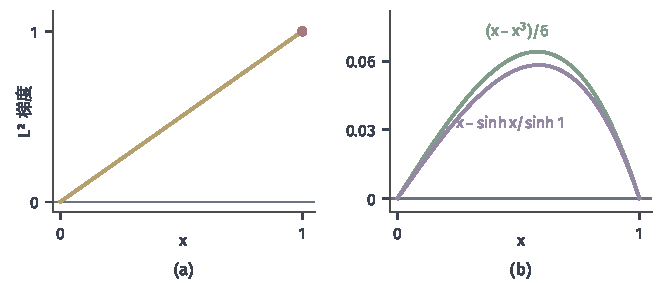
\includegraphics[width=112mm]{figures/05-optimization/08-functional-optimization/matplotlib/func-three-gradients/figure.pdf}
  \caption{$E$在$u=x$处同一微分的三个梯度。(a)$L^2$梯度$w_1=x$，在$x=1$处不为零（红点），不是允许的扰动方向。(b)绿色$w_2$对应内积$\int v'\eta'$，紫色$w_3$对应$H^1$内积，二者都在端点为零。注意两幅图的纵轴尺度相差十倍以上。}
  \label{fig:func-three-gradients}
\end{BookInlineFigure}

它们的差别有实际后果。$w_1$在$x=1$处等于$1$，沿它走一步会破坏端点条件，它不是$\bm{V}$中的元素：$\bm{V}$在$L^2$内积下不完备，Riesz定理在这里并没有保证梯度落在$\bm{V}$内。$w_2,w_3$是$\bm{V}$中的元素，沿它们走仍然可行。

$w_3$还有一个特别之处。$E$的二次项正是$H^1$内积，这和上面的$\bm{M}$取Hessian相同，所以$u-w_3=\sinh x/\sinh1$一步到位。这条曲线就是图~\ref{fig:func-feasible-directions}中绿色的候选，它的能量约为$0.6565$，比$E(x)=2/3$低；第~\ref{sec:func-integral}节将确认它就是极小点。

\paragraph{函数梯度与坐标梯度}
把函数离散成结点向量，函数的梯度与向量的梯度是什么关系？看最简单的$J(u)=\frac12\int_0^1u^2\,\mathrm{d}x$，它的$L^2$梯度是$u$。离散成$J_n(\bm{u})=\frac{\Delta}{2}\sum_iu_i^2$，向量梯度的分量是$\Delta u_i$，随网格加密趋于零。

要得到函数的梯度，必须除以$\Delta$。这正是式~\eqref{eq:func-metric-gradient}中取$\bm{M}=\Delta\bm{I}$，也就是离散$L^2$内积$\Delta\sum_iu_iv_i$。向量梯度依赖离散的细节，函数梯度依赖选定的内积，从前者到后者要乘以内积矩阵的逆。

\paragraph{梯度可以不存在}
有限维中，每个线性函数都连续，所以任何内积下都有梯度。无限维不是这样。考虑$E_0(u)=\frac12\int_0^1u'^2\,\mathrm{d}x$，在$\bm{V}=H^1_0(0,1)$的帐篷函数$u=\min\{x,1-x\}$处，把积分在$x=\frac12$处分开：
\[
 DE_0(u)[\eta]=\int_0^{1/2}\eta'\,\mathrm{d}x-\int_{1/2}^1\eta'\,\mathrm{d}x=2\,\eta\bigl(\tfrac12\bigr).
\]
微分只读取中点的值。在内积$\int v'\eta'$下，由定义，$\nabla E_0(u)=u$，这是图~\ref{fig:func-tent-gradient}(a)的帐篷。

在$L^2$内积下，$\eta\mapsto2\eta(\frac12)$不连续。取中点处高度为$1$、半宽为$1/k$的小帐篷$\eta_k$，有
\[
 DE_0(u)[\eta_k]=2,\qquad\lVert\eta_k\rVert_2^2=\frac{2}{3k}\to0.
\]
没有$L^2$函数能表示这个读取，$L^2$梯度不存在。形式上的“梯度”$-u''$是中点处质量为$2$的点质量，它不是函数。

把问题离散，就能看到这一点。线性元的结点向量梯度只在中点非零，等于$2$；转成离散$L^2$梯度要除以$\Delta=1/n$，于是高度为$2n$。图~\ref{fig:func-tent-gradient}(b)的尖峰随网格加密无限增高，没有极限函数。

\begin{BookInlineFigure}
  \centering
  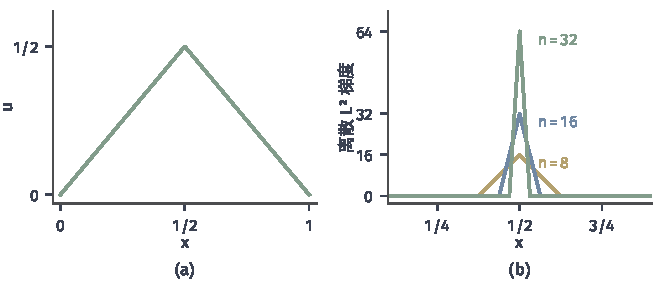
\includegraphics[width=112mm]{figures/05-optimization/08-functional-optimization/matplotlib/func-tent-gradient/figure.pdf}
  \caption{帐篷函数$u=\min\{x,1-x\}$在$E_0=\frac12\int u'^2\,\mathrm{d}x$下的梯度。(a)在内积$\int v'\eta'$下，梯度就是$u$本身。(b)离散$L^2$梯度，在$n=8,16,32$段网格上中点高度为$2n$，网格越细越高，没有极限函数。}
  \label{fig:func-tent-gradient}
\end{BookInlineFigure}

\paragraph{选错内积的代价}
即使$L^2$梯度存在，用它做下降也有问题。对式~\eqref{eq:func-energy}用$n$段线性元离散，在两种内积下跑步长为$1/L$的梯度下降，$L$是对应内积下的光滑常数。

$L^2$内积下，$L$约等于离散二阶差分的最大特征值$4n^2$。$n=16,32,64$时步长分别约为$9.9\times10^{-4}$、$2.4\times10^{-4}$、$6.1\times10^{-5}$，网格每加密一倍，步长缩小到四分之一。原因是$-u''$是无界的运算，函数摆动越快，它放大得越多。

内积$\int v'\eta'$下，相应的算子把频率$k$的分量放大$1+(k\pi)^{-2}$倍，$L\approx1.10$与网格无关。图~\ref{fig:func-gd-metric}显示了结果，绿线几步就到达机器精度，黄线$100$步后目标差仍在$10^{-3}$到$10^{-2}$之间，而且网格越细越慢。

\begin{BookInlineFigure}
  \centering
  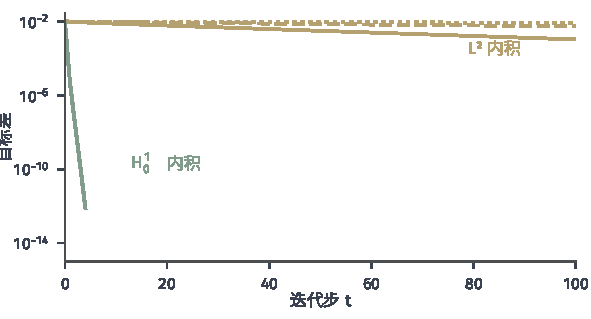
\includegraphics[width=100mm]{figures/05-optimization/08-functional-optimization/matplotlib/func-gd-metric/figure.pdf}
  \caption{线性元离散的$E$上，步长$1/L$的梯度下降从$u=x$出发的目标差。黄色为$L^2$内积，绿色为内积$\int v'\eta'$；实线、虚线、点线分别是$n=16,32,64$。绿色三条线重合，收敛不随网格变慢。}
  \label{fig:func-gd-metric}
\end{BookInlineFigure}

这和第~\ref{chap:second-order-methods}章讲的二阶信息是同一件事：选一个接近Hessian的内积，就是做预条件。函数空间的视角补充的是：网格加密时，好的内积让迭代次数保持不变，这件事在单个有限维问题里看不出来。

\paragraph{类比到哪里为止}
下面把向量与函数的对应关系补完，并列出类比失效的地方。

\begin{BookInlineTable}
  \centering
  \caption{一阶信息的对应与差别。}
  \label{tab:func-gradient-analogy}
  \begin{tabular}{lll}
    \toprule
    & 有限维 & 函数空间\\
    \midrule
    闭球 & 紧 & 不紧，只有弱序列紧\\
    范数 & 彼此等价 & 不等价，决定可微性\\
    线性泛函 & 自动连续 & 可以不连续\\
    梯度 & 任何内积下都存在 & 可能不存在\\
    Hessian & 有界 & 在 $L^2$ 中可以无界\\
    \bottomrule
  \end{tabular}
\end{BookInlineTable}

可以这样记：有限维的直觉在选定空间之后才能使用，选空间这一步是函数问题特有的。

\section{最优解的判别}
\label{sec:func-optimality}

有了微分，就可以判别候选。泛函优化的最优解满足什么条件，什么条件又足以断定最优？一阶条件、凸性下的充分性与有限维完全平行；二阶充分性和约束乘子则要额外的前提。

\paragraph{局部极小依赖范数}
在讲条件之前要先说清“局部”。设$J$定义在$\bm{C}$上，若存在$r>0$，使$\lVert u-u^\star\rVert<r$的可行$u$都满足$J(u)\geq J(u^\star)$，称$u^\star$是范数$\lVert\cdot\rVert$下的\term{局部极小点}（local minimizer）。有限维中范数等价，不用说明是哪一个；函数空间中必须说明。

看下面的例子。在$[0,1]$上的Lipschitz函数中，取$u(0)=u(1)=0$，目标
\begin{equation}
 J(u)=\int_0^1\bigl(u'(x)^2-u'(x)^4\bigr)\,\mathrm{d}x.
 \label{eq:func-local-example}
\end{equation}
若用范数$\lVert u\rVert_\infty+\lVert u'\rVert_\infty$，当它小于$1$时$\lvert u'\rvert<1$，被积函数非负，$J\geq0=J(0)$，所以$u=0$是局部极小点。

若只用上确界范数$\lVert u\rVert_\infty$，取图~\ref{fig:func-zigzag-local}(a)的锯齿：$k$个相同的齿，斜率$\pm2$。它的高度是$1/k$，$k$越大越贴近零函数；而被积函数处处等于$4-16=-12$，
\[
 \lVert u\rVert_\infty=\frac1k,\qquad J(u)=-12.
\]
所以$u=0$在上确界范数下不是局部极小点。前一种范数把导数也算进“接近”，这样的扰动被排除了。

\begin{BookInlineFigure}
  \centering
  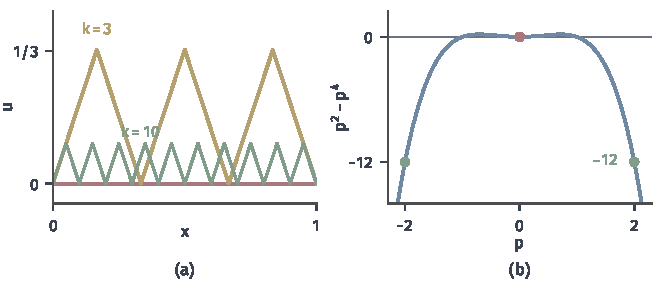
\includegraphics[width=112mm]{figures/05-optimization/08-functional-optimization/matplotlib/func-zigzag-local/figure.pdf}
  \caption{局部极小依赖范数。(a)红线$u=0$附近的锯齿，斜率$\pm2$，黄色$k=3$，绿色$k=10$；上确界距离$1/k$趋于零，而导数始终等于$\pm2$。(b)被积函数$p^2-p^4$：$p=0$是局部极小（红点），大斜率处（绿点）取值$-12$。}
  \label{fig:func-zigzag-local}
\end{BookInlineFigure}

\paragraph{一阶必要条件}
第~\ref{chap:constrained-optimality}章用可行方向得到一阶条件，这里的推理逐字相同，因为它只看一条线段。称$\eta$是$\bm{C}$在$u$处的\term{可行方向}（feasible direction），若$t>0$充分小时$u+t\eta\in\bm{C}$。

\begin{theorem}[一阶必要条件]
\label{thm:func-first-order}
设$u^\star$是$J$在$\bm{C}$上某范数下的局部极小点，$\eta$是$u^\star$处的可行方向，方向导数存在。则
\begin{equation}
 J'(u^\star;\eta)\geq0.
 \label{eq:func-first-order}
\end{equation}
进一步，设$J$在$u^\star$处沿所需方向Gâteaux可微。若$\bm{C}=u_0+\bm{V}$，$\bm{V}$是子空间，则
\begin{equation}
 DJ(u^\star)[\eta]=0\qquad(\eta\in\bm{V}).
 \label{eq:func-stationary}
\end{equation}
若$\bm{C}$是凸集，则
\begin{equation}
 DJ(u^\star)[v-u^\star]\geq0\qquad(v\in\bm{C}).
 \label{eq:func-variational-inequality}
\end{equation}
\end{theorem}

\begin{proof}
$t>0$充分小时，$u^\star+t\eta$可行，且与$u^\star$的距离$t\lVert\eta\rVert$小于$r$，所以
\[
 \frac{J(u^\star+t\eta)-J(u^\star)}{t}\geq0.
\]
令$t\downarrow0$得到式~\eqref{eq:func-first-order}。子空间情形中$\eta$和$-\eta$都是可行方向，由线性得到两个相反的不等式，于是式~\eqref{eq:func-stationary}成立。凸集情形中$v-u^\star$是可行方向，代入式~\eqref{eq:func-first-order}。
\end{proof}

式~\eqref{eq:func-stationary}称为驻定条件，满足它的点称为驻点。若$\bm{V}$上有Hilbert结构，它就是$\nabla_{\bm{V}}J(u^\star)=0$。注意这里的梯度是$\bm{V}$内的，$X$内的梯度只需与$\bm{V}$正交，这和等式约束问题中梯度落在约束法方向上相同。式~\eqref{eq:func-variational-inequality}是第~\ref{chap:constrained-optimality}章的变分不等式。

\paragraph{凸性下的充分性}
凸性让局部信息变成全局结论。若$J$是凸泛函，沿线段的一元函数$\phi$是凸的，切线在下方，由此得到下面的结论。

\begin{theorem}[凸问题的充分条件]
\label{thm:func-convex-sufficient}
设$\bm{C}$是凸集，$J$在$\bm{C}$上是凸的，在$u^\star\in\bm{C}$处有$J'(u^\star;v-u^\star)\geq0$，对每个$v\in\bm{C}$成立。则$u^\star$是全局最优解。若$J$严格凸，它是唯一的最优解。
\end{theorem}

\begin{proof}
任取$v\in\bm{C}$，令$\phi(t)=J(u^\star+t(v-u^\star))$，$t\in[0,1]$。由凸性，$t\in(0,1]$时
\[
 \frac{\phi(t)-\phi(0)}{t}\leq\phi(1)-\phi(0).
\]
令$t\downarrow0$，左端趋于$J'(u^\star;v-u^\star)\geq0$，所以$J(v)\geq J(u^\star)$。

若$J$严格凸，并有另一最优解$v\neq u^\star$，则中点的目标值严格小于$J^\star$，矛盾。
\end{proof}

对$E$，式~\eqref{eq:func-energy-expansion}中的余项$\frac12\lVert\eta\rVert_{H^1}^2$在$\eta\neq0$时严格为正。所以$E$严格凸，驻点若存在，就是唯一的全局最优解。第~\ref{sec:func-existence}节证明了存在性，这里证明了驻点即最优，两者合起来，驻定方程的解就是答案。

\paragraph{二阶变化}
没有凸性时，要看二阶信息。沿直线，$\phi''(0)$就是二阶变化。

\begin{definition}[二阶变分]
\label{def:func-second-variation}
若$\phi(t)=J(u+t\eta)$在$t=0$的邻域内二阶可导，称
\begin{equation}
 \delta^2J(u;\eta)=\phi''(0)
 \label{eq:func-second-variation}
\end{equation}
为$J$在$u$处沿$\eta$的\term{二阶变分}（second variation）。
\end{definition}

若$u^\star$是子空间方向上的局部极小点，则$\phi$在$t=0$处局部极小，所以$\phi'(0)=0$，并有$\phi''(0)\geq0$。这是二阶必要条件：$\delta^2J(u^\star;\eta)\geq0$，对每个$\eta\in\bm{V}$成立。

\paragraph{用坐标看二阶变分}
目标~\eqref{eq:func-rho}是二次的，$\phi(t)=t^2J_\rho(\eta)$，所以
\[
 \delta^2J_\rho(0;\eta)=\int_0^1\bigl(\eta'^2-\rho\eta^2\bigr)\,\mathrm{d}x.
\]
把$\eta\in H^1_0(0,1)$按标准正交基$\sqrt2\sin(k\pi x)$展开，系数为$a_k$。由Parseval等式，$\lVert\eta\rVert_2^2=\sum_ka_k^2$。

对$\eta'$，它按$\sqrt2\cos(k\pi x)$展开的系数，由分部积分（边界项因$\eta$在端点为零而消失）等于$k\pi a_k$；它与常数函数的内积是$\eta(1)-\eta(0)=0$。所以$\lVert\eta'\rVert_2^2=\sum_k(k\pi)^2a_k^2$。三角函数系的完备性可参考\BookChapterRef{chap:fourier-transform}{卷四第14章“Fourier变换”}。代入得到
\begin{equation}
 \delta^2J_\rho(0;\eta)=\sum_{k=1}^\infty\bigl((k\pi)^2-\rho\bigr)a_k^2.
 \label{eq:func-spectrum}
\end{equation}

这是无限维中的对角二次型，图~\ref{fig:func-spectrum}(a)是$\rho=15$时的对角元。只有$k=1$为负，所以$u=0$是鞍点。对角元有下界但无上界，这是有限维Hessian没有的现象：图~\ref{fig:func-spectrum}(b)中，把问题离散后，最大特征值约为$4n^2$，随网格加密趋于无穷，最小特征值停在$\pi^2$附近。

\begin{BookInlineFigure}
  \centering
  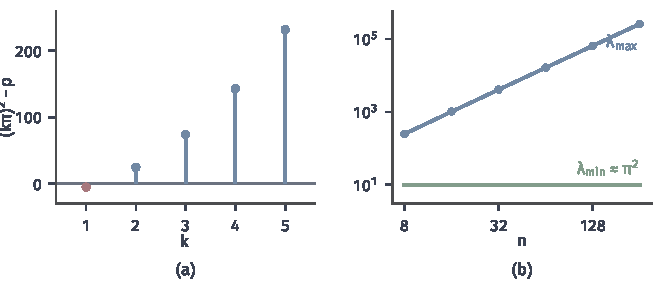
\includegraphics[width=112mm]{figures/05-optimization/08-functional-optimization/matplotlib/func-spectrum/figure.pdf}
  \caption{目标~\eqref{eq:func-rho}的二阶信息。(a)$\rho=15$时式~\eqref{eq:func-spectrum}的对角元，红色为负曲率方向$k=1$。(b)二阶差分矩阵的最大特征值（蓝）随段数$n$按$4n^2$增长，最小特征值（绿）停在$\pi^2$附近，所以$L^2$意义下没有有限的光滑常数$L$。}
  \label{fig:func-spectrum}
\end{BookInlineFigure}

由式~\eqref{eq:func-spectrum}可以读出全部结论。$\rho<\pi^2$时每个对角元为正，$J_\rho$严格凸，$u=0$是唯一的最优解。$\rho=\pi^2$时$t\sin\pi x$全是最优解，解不唯一。$\rho>\pi^2$时目标无下界。这也给出了精确的Poincaré不等式：
\[
 \lVert\eta'\rVert_2^2\geq\pi^2\lVert\eta\rVert_2^2.
\]

\paragraph{处处为正不够}
有限维中，Hessian正定就足以保证严格局部极小，因为单位球面紧，正定函数在其上有正的最小值$\mu$。无限维中球面不紧，这个最小值可以是$0$。

在$\ell^2$上，也就是把函数看成坐标序列，令
\[
 J(\bm{a})=\sum_{k=1}^\infty\Bigl(\frac{a_k^2}{k^2}-a_k^4\Bigr).
\]
由$\sum_ka_k^4\leq\lVert\bm{a}\rVert_2^4$，$J$处处有限。在原点，$J$的一阶微分为零，二阶变分$\delta^2J(\bm{0};\bm{\eta})=2\sum_k\eta_k^2/k^2$，对每个$\bm{\eta}\neq\bm{0}$都是正的。

但取只有第$k$个坐标非零的点$\bm{a}^{(k)}=\frac2k\bm{e}_k$，有
\[
 \lVert\bm{a}^{(k)}\rVert_2=\frac2k\to0,\qquad J(\bm{a}^{(k)})=\frac{4}{k^4}-\frac{16}{k^4}=-\frac{12}{k^4}<0.
\]
所以原点不是局部极小点。曲率$2/k^2$沿高频坐标趋于零，四次项就占了上风。要恢复有限维的结论，必须要求曲率有统一的正下界。

\begin{theorem}[二阶充分条件]
\label{thm:func-second-sufficient}
设$\bm{C}=u_0+\bm{V}$，$J$在$u^\star\in\bm{C}$的邻域内二阶连续Fréchet可微，$DJ(u^\star)$在$\bm{V}$上为零，且存在$\mu>0$使
\begin{equation}
 D^2J(u^\star)[\eta,\eta]\geq\mu\lVert\eta\rVert^2\qquad(\eta\in\bm{V}).
 \label{eq:func-coercive-second}
\end{equation}
则$u^\star$是所用范数下的严格局部极小点。
\end{theorem}

\begin{proof}
由连续性，取$r>0$，使$\lVert v-u^\star\rVert<r$时$\lVert D^2J(v)-D^2J(u^\star)\rVert\leq\mu/2$。对$\eta\in\bm{V}$，$0<\lVert\eta\rVert<r$，用带积分余项的Taylor公式，一阶项为零，
\[
 J(u^\star+\eta)-J(u^\star)=\int_0^1(1-\tau)D^2J(u^\star+\tau\eta)[\eta,\eta]\,\mathrm{d}\tau.
\]
被积式中的二阶微分不小于$\mu\lVert\eta\rVert^2-\frac\mu2\lVert\eta\rVert^2$，所以
\[
 J(u^\star+\eta)-J(u^\star)\geq\frac{\mu}{4}\lVert\eta\rVert^2>0.
\]
\end{proof}

上面的$\ell^2$反例不满足式~\eqref{eq:func-coercive-second}。而$J_\rho$在$0\le\rho<\pi^2$时满足它：由式~\eqref{eq:func-spectrum}，在范数$\lVert\eta'\rVert_2$下，$\mu=1-\rho/\pi^2$。条件是否成立同样依赖范数：同一个二阶变分在$H^1$范数下是强制的，在更强的范数下可能不是。

\paragraph{约束乘子}
若约束不是仿射的，第~\ref{chap:constrained-optimality}章的乘子法则还成立吗？有限个约束时答案是肯定的，因为证明可以化归到有限维。

\begin{theorem}[有限个等式约束的乘子法则]
\label{thm:func-multiplier}
设$X$是Banach空间，$u^\star$是$J$在约束$h_j(u)=0$（$j=1,\ldots,p$）下某范数的局部极小点。设$J,h_1,\ldots,h_p$在$u^\star$的邻域内连续Fréchet可微，且$Dh_1(u^\star),\ldots,Dh_p(u^\star)$线性无关。则存在唯一的$\bm{\nu}\in\mathbb{R}^p$，使
\begin{equation}
 DJ(u^\star)+\sum_{j=1}^p\nu_jDh_j(u^\star)=0\quad\text{于}\ X^*.
 \label{eq:func-multiplier}
\end{equation}
\end{theorem}

\begin{proof}
\emph{选取补方向。}由线性无关，存在$e_1,\ldots,e_p\in X$，使$Dh_i(u^\star)[e_j]$当$i=j$时为$1$，否则为$0$。记$\bm{N}$为全部$Dh_j(u^\star)$的公共零空间。

\emph{化到有限维。}固定$\eta\in\bm{N}$，考虑从$\mathbb{R}\times\mathbb{R}^p$到$\mathbb{R}^p$的映射
\[
 \Psi_j(t,\bm{s})=h_j\Bigl(u^\star+t\eta+\sum_{i=1}^ps_ie_i\Bigr).
\]

在原点$\bm{\Psi}$取零，对$\bm{s}$的Jacobi矩阵是单位阵。由隐函数定理，存在$\bm{s}(0)=\bm{0}$的$C^1$函数$\bm{s}(t)$，使约束沿$t$始终成立。

对$t$求导，并用$Dh_j(u^\star)[\eta]=0$，得到
\[
 \bm{s}'(0)=\bm{0}.
\]

\emph{沿可行曲线求导。}令$w(t)=u^\star+t\eta+\sum_is_i(t)e_i$，它可行，$w(0)=u^\star$，$w'(0)=\eta$。一元函数$J(w(t))$在$t=0$处局部极小，所以导数为零，即$DJ(u^\star)[\eta]=0$。

\emph{写出乘子。}令$\nu_j=-DJ(u^\star)[e_j]$。对任意$v\in X$，$v-\sum_jDh_j(u^\star)[v]\,e_j$属于$\bm{N}$，代入上一步得到
\[
 DJ(u^\star)[v]=-\sum_{j=1}^p\nu_jDh_j(u^\star)[v].
\]
这就是式~\eqref{eq:func-multiplier}。唯一性由线性无关得到。
\end{proof}

关键在于约束只有有限个，隐函数定理只用在$\mathbb{R}^p$上。条件中的连续Fréchet可微和线性无关都依赖所选的空间。

\paragraph{一个可以手算的乘子}
一根两端固定的细线绕过中点处高度为$1$的钉子。写成问题，就是
\[
 \min\ \frac12\int_0^1u'(x)^2\,\mathrm{d}x,\qquad u\in H^1_0(0,1),\quad u(\tfrac12)\geq1.
\]
点值读取在$H^1$中连续，由式~\eqref{eq:func-point-bound}，这个约束是良定义的。候选是图~\ref{fig:func-peg}(a)的折线$u^\star=2\min\{x,1-x\}$。

直接计算微分：把积分在$x=\frac12$处分开，
\[
 DJ(u^\star)[\eta]=2\int_0^{1/2}\eta'\,\mathrm{d}x-2\int_{1/2}^1\eta'\,\mathrm{d}x=4\,\eta\bigl(\tfrac12\bigr).
\]
可行集是凸集。对可行的$v$，有$v(\frac12)\geq1=u^\star(\frac12)$，所以
\[
 DJ(u^\star)[v-u^\star]=4\bigl(v(\tfrac12)-1\bigr)\geq0.
\]
由定理~\ref{thm:func-convex-sufficient}，$u^\star$是全局最优解，$J^\star=\frac12\cdot4=2$。

\begin{BookInlineFigure}
  \centering
  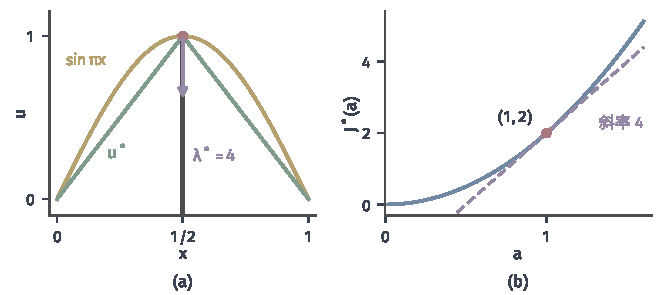
\includegraphics[width=112mm]{figures/05-optimization/08-functional-optimization/matplotlib/func-peg/figure.pdf}
  \caption{钉子问题。(a)深灰竖线是钉子，绿色折线是最优解，黄色$\sin\pi x$是另一个可行候选（能量$\pi^2/4\approx2.47$，大于$2$），紫色箭头表示乘子$\lambda^\star=4$。(b)钉子高度为$a$时的最优值$J^\star(a)=2a^2$，$a=1$处切线（紫色虚线）的斜率等于乘子。}
  \label{fig:func-peg}
\end{BookInlineFigure}

把约束写成$g(u)=1-u(\frac12)\leq0$，于是$Dg[\eta]=-\eta(\frac12)$。平稳条件$DJ(u^\star)+\lambda Dg=0$给出乘子
\[
 \lambda^\star=4\geq0.
\]
乘子仍是影子价格。钉子高度为$a$时，最优解是$2a\min\{x,1-x\}$，最优值是$J^\star(a)=2a^2$，在$a=1$处的导数正是$4$，见图~\ref{fig:func-peg}(b)。把高度抬高一点，能量按每单位高度$4$增加。

这个乘子也可以用梯度来读。在内积$\int v'\eta'$下，读取$\eta\mapsto\eta(\frac12)$的梯度是$w=\frac12\min\{x,1-x\}$，因为$\int_0^1w'\eta'\,\mathrm{d}x=\eta(\frac12)$。而$\nabla J(u^\star)=u^\star=4w$。目标的梯度等于乘子乘以约束的梯度，这与有限维的几何完全相同。

\paragraph{乘子的适用前提}
上面的例子只有一个约束。若要求$u(x)\geq\psi(x)$对每个$x$成立，约束就有无穷多个，定理~\ref{thm:func-multiplier}用不上。乘子要变成对偶空间中的元素，它通常不是函数。把钉子看成这种情形，乘子是中点处的点质量$4\delta_{1/2}$，$u'$在钉子处恰好跳变$-4$。

无穷约束下乘子的存在，需要Slater型条件，也就是可行集在合适拓扑中有内点。这时拓扑的选择又起决定作用：$L^2$中非负函数组成的锥没有内点，因为从任何非负函数减去一个窄而高的尖峰，都可以用任意小的$L^2$范数变成在一小段上为负。而$C[0,1]$中$u\geq\varepsilon>0$的函数是内点。一维时$H^1$的范数控制上确界，内点也存在；高维时这一点不再成立，需要在具体问题中重新论证。

所以，有限维的乘子法则搬到函数空间时要检查三件事：约束是有限个还是无穷个，约束在所选范数下是否可微，约束规范在所选拓扑下是否成立。

\section{积分泛函}
\label{sec:func-integral}

前几节的目标$E$和$\ell$都是沿区间累加一个局部代价。于是要问：对这一类目标，最优性条件具体是什么？答案是一个常微分方程，加上由约束决定的边界条件。

设$F(x,s,p)$是定义在$[a,b]\times\mathbb{R}\times\mathbb{R}$上的函数，称为\term{密度}（density），对$(s,p)$连续可微，偏导数连续。\term{积分泛函}（integral functional）是
\begin{equation}
 J(u)=\int_a^bF\bigl(x,u(x),u'(x)\bigr)\,\mathrm{d}x.
 \label{eq:func-integral}
\end{equation}
下面用$F_s,F_p$表示$F$对第二、第三个变量的偏导数，沿候选求值时省略自变量，即$F_p$表示$F_p(x,u(x),u'(x))$，它是$x$的函数。$F_p$是对“斜率所在的变量”求偏导，不是对函数$u'$求导。

\paragraph{一阶变分}
沿直线$u+t\eta$求导，只需把导数换到积分号内。

\begin{theorem}[积分泛函的一阶变分]
\label{thm:func-first-variation}
设$u,\eta\in C^1[a,b]$。则
\begin{equation}
 J'(u;\eta)=\int_a^b\bigl(F_s\,\eta+F_p\,\eta'\bigr)\,\mathrm{d}x.
 \label{eq:func-first-variation}
\end{equation}
\end{theorem}

\begin{proof}
函数$(x,t)\mapsto F(x,u+t\eta,u'+t\eta')$对$t$的偏导数是$F_s\eta+F_p\eta'$在点$(x,u+t\eta,u'+t\eta')$的值，它在紧集$[a,b]\times[-1,1]$上连续。连续偏导数允许在积分号下求导，令$t=0$即得。
\end{proof}

这也是方向导数的线性公式。$J'(u;\eta)$对$\eta$线性，并被$\eta$的$C^1$范数控制。对Sobolev函数，要在积分号下求导还需要控制收敛定理所要求的可积上界，要根据$F$的增长条件逐项核对；$E$和$\ell$的情形已由第~\ref{sec:func-directional}节的展开直接得到。

\subsection{Euler--Lagrange方程}
\label{sec:func-euler-lagrange}

\paragraph{用分部积分消去$\eta'$}
一阶变分同时含$\eta$和$\eta'$，而它们不是独立的。为了让式子只含$\eta$，把$\eta'$前的系数移走。设$u\in C^2[a,b]$，$F$二阶连续可微，分部积分得到
\begin{equation}
 J'(u;\eta)=\int_a^b\Bigl(F_s-\frac{\mathrm{d}}{\mathrm{d}x}F_p\Bigr)\eta\,\mathrm{d}x+\Bigl[F_p\,\eta\Bigr]_a^b.
 \label{eq:func-first-variation-parts}
\end{equation}
边界项先记下来。固定端点时，可行扰动在两端为零，边界项消失。第~\ref{sec:func-free-boundary}小节放开端点时，这一项会成为主角。

此时括号里的函数在$L^2$内积下正是$J$的梯度。由第~\ref{sec:func-hilbert-gradient}小节，$E$在$u=x$处的$L^2$梯度是$x$，这里$-u''+u=x$，两者一致。驻定条件要求这个梯度与所有扰动正交，接下来把“正交于所有扰动”变成“等于零”。

\paragraph{变分基本引理}
在有限维中，若$\bm{g}^\top\bm{d}=0$对每个$\bm{d}$成立，取$\bm{d}=\bm{g}$得$\bm{g}=\bm{0}$。函数空间里扰动有端点和光滑性要求，不能直接取$\eta=g$，但可以取一个局部的小凸起，见图~\ref{fig:func-bump-lemma}。

\begin{lemma}[变分基本引理]
\label{lem:func-fundamental}
设$g\in C[a,b]$，且对每个在$(a,b)$内紧支撑的光滑函数$\eta$都有$\int_a^bg\,\eta\,\mathrm{d}x=0$。则$g\equiv0$。
\end{lemma}

\begin{proof}
设有$x_0\in(a,b)$使$g(x_0)>0$，$g(x_0)<0$的情形相同。由连续性，存在$r>0$，使$(x_0-r,x_0+r)\subset(a,b)$，且$g$在其上为正。取$\eta$为支撑在这个区间内的非负光滑函数，例如当$\lvert x-x_0\rvert<r$时
\[
 \eta(x)=\exp\Bigl(\frac{-1}{1-(x-x_0)^2/r^2}\Bigr),
\]
其余位置为零。则$g\eta\geq0$，在$x_0$处严格为正，于是积分为正，与假设矛盾。所以$g$在$(a,b)$内为零，由连续性在端点也为零。
\end{proof}

\begin{BookInlineFigure}
  \centering
  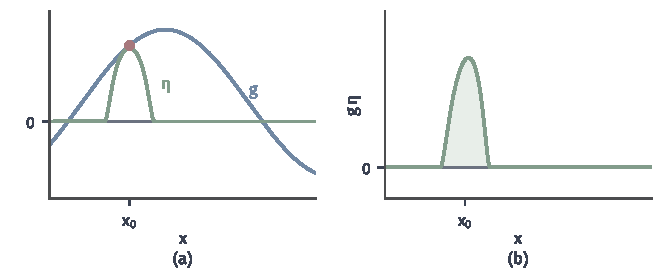
\includegraphics[width=112mm]{figures/05-optimization/08-functional-optimization/matplotlib/func-bump-lemma/figure.pdf}
  \caption{变分基本引理的构造。(a)蓝色$g$在红点$x_0$处为正，绿色凸起$\eta$只在$g>0$的小区间内非零。(b)乘积$g\eta$非负，积分严格为正，所以$g$不能与所有扰动正交。}
  \label{fig:func-bump-lemma}
\end{BookInlineFigure}

把扰动限制在局部，等于“单独改动一小段曲线”。这是向量情形“单独改动一个坐标”的连续版本：极小点处每一小段都不能再改进，方程因此对每个$x$成立。

\begin{theorem}[Euler--Lagrange方程]
\label{thm:func-euler-lagrange}
设$F$二阶连续可微，$u\in C^2[a,b]$满足$u(a)=\alpha$，$u(b)=\beta$，并且在固定端点的$C^1$函数中，是$C^1$范数下$J$的局部极小点。则对每个$x\in[a,b]$，
\begin{equation}
 \frac{\mathrm{d}}{\mathrm{d}x}F_p\bigl(x,u(x),u'(x)\bigr)=F_s\bigl(x,u(x),u'(x)\bigr).
 \label{eq:func-euler-lagrange}
\end{equation}
\end{theorem}

\begin{proof}
可行方向是端点为零的$C^1$函数，它们组成子空间，由定理~\ref{thm:func-first-order}得$J'(u;\eta)=0$。式~\eqref{eq:func-first-variation-parts}的边界项为零，再由引理~\ref{lem:func-fundamental}，括号内的连续函数恒为零。
\end{proof}

式~\eqref{eq:func-euler-lagrange}称为\term{Euler--Lagrange方程}（Euler--Lagrange equation），它的解称为\term{极值曲线}（extremal）。这个名称有些误导，因为解不一定是极值，下面专门讨论这一点。

\paragraph{两个例子}
对长度目标~\eqref{eq:func-length}，$F=\sqrt{1+p^2}$不依赖$s$，所以$F_s=0$，方程~\eqref{eq:func-euler-lagrange}说$F_p$是常数：
\[
 \frac{u'(x)}{\sqrt{1+u'(x)^2}}=c.
\]
函数$p\mapsto p/\sqrt{1+p^2}$严格递增，所以$u'$是常数，$u$是直线。加上端点条件得$u(x)=x$，$\ell^\star=\sqrt2$。

对能量~\eqref{eq:func-energy}，$F=\frac12p^2+\frac12s^2$，$F_p=p$，$F_s=s$，方程是
\begin{equation}
 u''=u,\qquad u(0)=0,\ u(1)=1.
 \label{eq:func-energy-el}
\end{equation}
通解是$A\sinh x+B\cosh x$，由$u(0)=0$得$B=0$，由$u(1)=1$得$A=1/\sinh1$，于是
\begin{equation}
 u^\star(x)=\frac{\sinh x}{\sinh1}.
 \label{eq:func-energy-solution}
\end{equation}
这就是第~\ref{sec:func-hilbert-gradient}小节由一步梯度得到的曲线。由$u''=u$，有$u'^2+u^2=(uu')'$，积分得到最优值
\begin{equation}
 E^\star=\frac12\bigl[uu'\bigr]_0^1=\frac12u'(1)=\frac12\coth1\approx0.6565.
 \label{eq:func-energy-value}
\end{equation}
$E$严格凸，由定理~\ref{thm:func-convex-sufficient}，$u^\star$就是唯一的全局最优解。

\paragraph{函数要有多光滑}
推导用了$u\in C^2$，它只是为了分部积分。候选只有$C^1$时，换一个方向分部积分，把导数放到$F_s$的原函数上。令$A(x)=\int_a^xF_s\,\mathrm{d}\tau$，它是$C^1$函数。分部积分，由$\eta$在端点为零得到
\[
 \int_a^bF_s\eta\,\mathrm{d}x=-\int_a^bA\eta'\,\mathrm{d}x.
\]
于是驻定条件变成
\[
 \int_a^b(F_p-A)\,\eta'\,\mathrm{d}x=0\qquad\text{对端点为零的}\ \eta\in C^1.
\]

下面的引理把这个条件化成$F_p-A$是常数。设$g\in C[a,b]$满足$\int_a^bg\eta'\,\mathrm{d}x=0$。令$c$为$g$的平均值，取$\eta(x)=\int_a^x(g-c)\,\mathrm{d}\tau$，它在两端为零，由$\int_a^b\eta'\,\mathrm{d}x=0$得到
\[
 \int_a^b(g-c)^2\,\mathrm{d}x=\int_a^b(g-c)\eta'\,\mathrm{d}x=\int_a^bg\eta'\,\mathrm{d}x=0.
\]
所以$g\equiv c$。这一结论称为du Bois-Reymond引理。把它用在$g=F_p-A$上，得到积分形式的方程
\begin{equation}
 F_p\bigl(x,u(x),u'(x)\bigr)=c+\int_a^xF_s\,\mathrm{d}\tau.
 \label{eq:func-du-bois}
\end{equation}
右端是$C^1$的，所以$F_p$沿曲线可导且满足式~\eqref{eq:func-euler-lagrange}，虽然$u''$可能不存在。若$F_{pp}>0$，由隐函数定理可从$F_p$解出$u'$，$u$自动属于$C^2$。

式~\eqref{eq:func-du-bois}对分段$C^1$的候选同样成立，而右端连续，所以在曲线的折点处，$F_p$不能跳变。这是极值曲线可以有折点的唯一条件。对$G(p)=(p^2-1)^2$，$F_p=4p(p^2-1)$在$p=\pm1$处都为零，所以斜率$\pm1$的锯齿满足这个条件。而钉子问题中$F_p=u'$在中点跳变，因为那里的扰动受到约束，驻定条件只对$\eta(\frac12)=0$的方向成立，跳变的幅度$4$正是乘子。

对$H^1$中的极小点，能直接得到的只有弱形式：$\int_a^b(F_s\eta+F_p\eta')\,\mathrm{d}x=0$。极小点是否足够光滑从而满足方程的经典形式，是方程理论的正则性问题，可参考\BookChapterRef{chap:elliptic-equations}{卷六第7章“椭圆方程”}。

\paragraph{方程是必要条件}
式~\eqref{eq:func-euler-lagrange}由“若是局部极小点”推出，反过来不成立。对目标~\eqref{eq:func-rho}，$F_p=p$，$F_s=-\rho s$，方程是$u''+\rho u=0$，$u=0$总是解。而第~\ref{sec:func-optimality}节已经算出，$\rho>\pi^2$时$u=0$是鞍点，目标甚至无下界。

要断定一个解是极小点，有两条路。若$F$对$(s,p)$联合凸，则$J$是凸泛函，由定理~\ref{thm:func-convex-sufficient}，满足端点条件和方程的$u$就是全局最优解，这是$E$和$\ell$的情形。没有凸性时，要检查二阶变分，它的积分形式是
\begin{equation}
 \delta^2J(u;\eta)=\int_a^b\bigl(F_{ss}\,\eta^2+2F_{sp}\,\eta\eta'+F_{pp}\,\eta'^2\bigr)\,\mathrm{d}x.
 \label{eq:func-second-variation-integral}
\end{equation}

\paragraph{二阶必要条件的局部形式}
式~\eqref{eq:func-second-variation-integral}中哪一项决定符号？取一个窄的帐篷形扰动，半宽和高度都是$\varepsilon$，斜率为$\pm1$。$\eta^2$项的量级是$\varepsilon^3$，$\eta\eta'$项是$\varepsilon^2$，$\eta'^2$项是$\varepsilon$。$\varepsilon$很小时，$F_{pp}$的项占主导，高频扰动只看得见$F_{pp}$。

\begin{theorem}[Legendre条件]
\label{thm:func-legendre}
设$F$二阶连续可微，$u\in C^1[a,b]$是固定端点问题在$C^1$范数下的局部极小点。则对每个$x\in[a,b]$，
\begin{equation}
 F_{pp}\bigl(x,u(x),u'(x)\bigr)\geq0.
 \label{eq:func-legendre}
\end{equation}
\end{theorem}

\begin{proof}
设在内点$x_0$处$F_{pp}<0$，端点的情形由连续性归结到内点。由连续性，存在$c>0$和$\varepsilon_0>0$，使$\lvert x-x_0\rvert\leq\varepsilon_0$时$F_{pp}\leq-c$。对$\varepsilon<\varepsilon_0$取上述帐篷形扰动，把折点磨圆使之成为$C^1$函数，磨圆可以使下列估计的改变任意小。由式~\eqref{eq:func-second-variation-integral}，存在只依赖$F$和$u$的常数$M$，使
\[
 \delta^2J(u;\eta)\leq-2c\,\varepsilon+M\varepsilon^2.
\]
$\varepsilon$足够小时右端为负，与二阶必要条件矛盾。
\end{proof}

对目标~\eqref{eq:func-bolza}，$G''(0)=-4<0$，所以$u=0$不是局部极小点，这与第~\ref{sec:func-existence}节的观察一致：$G$在$0$附近非凸，锯齿能把目标压低。Legendre条件仍只是必要的。目标~\eqref{eq:func-local-example}在$u=0$处$F_{pp}=2>0$，$u=0$在$C^1$范数下也确实是局部极小点，但在上确界范数下不是。

\paragraph{向量值函数与多元区域}
方程可以逐分量推广。若未知量是向量值函数$\bm{u}:[a,b]\to\mathbb{R}^r$，密度为$F(x,\bm{s},\bm{p})$，每次只扰动一个分量，重复上面的论证，得到方程组
\begin{equation}
 \frac{\mathrm{d}}{\mathrm{d}x}\nabla_{\bm{p}}F=\nabla_{\bm{s}}F.
 \label{eq:func-euler-lagrange-vector}
\end{equation}
若未知量是区域$\Omega\subset\mathbb{R}^d$上的函数，目标是
\[
 J(u)=\int_\Omega F(\bm{x},u,\nabla u)\,\mathrm{d}\bm{x},
\]
分部积分换成散度定理，方程变为
\begin{equation}
 \operatorname{div}\bigl(\nabla_{\bm{p}}F\bigr)=F_s.
 \label{eq:func-euler-lagrange-div}
\end{equation}
例如$F=\frac12\lVert\bm{p}\rVert_2^2-g(\bm{x})s$给出$-\Delta u=g$。这些方程的解的理论不属于本章。

\subsection{自由边界条件}
\label{sec:func-free-boundary}

至此端点都是固定的。若端点可以移动，可行扰动就变多了，最优解要多满足一些条件。本小节要回答的问题是：多出来的扰动告诉我们什么？关键是重新核对式~\eqref{eq:func-first-variation-parts}中的边界项。

\paragraph{放开一个端点的值}
把例子改成：保留$u(1)=1$，$u(0)$不作约束。候选在$\bm{C}=\{u\in H^1(0,1):u(1)=1\}$中，扰动只需$\eta(1)=0$。设$u\in C^2$是极小点，推理分两步。

第一步，固定端点的扰动仍然允许。取两端为零的$\eta$，同样得到内部方程~\eqref{eq:func-euler-lagrange}，$u$仍满足它。第二步，把这个结论代回式~\eqref{eq:func-first-variation-parts}，积分项消失，只剩边界项。由$\eta(1)=0$，
\[
 0=J'(u;\eta)=\bigl[F_p\eta\bigr]_0^1=-F_p\bigl(0,u(0),u'(0)\bigr)\,\eta(0).
\]
$\eta(0)$可以取任意值，所以
\begin{equation}
 F_p\bigl(0,u(0),u'(0)\bigr)=0.
 \label{eq:func-natural}
\end{equation}

这样的条件称为\term{自然边界条件}（natural boundary condition），它不是提问时写下的，而是由优化自己产生的。若继续沿用固定端点的公式，方程少一个边界条件，解就不确定。第二步的逻辑也不能颠倒：必须先用内部扰动消去积分项，边界项才能单独出现。

对$E$，$F_p=u'$，条件是$u'(0)=0$。方程$u''=u$加上$u'(0)=0$，$u(1)=1$，解得
\begin{equation}
 u^\star(x)=\frac{\cosh x}{\cosh1}.
 \label{eq:func-free-solution}
\end{equation}
同样用$u'^2+u^2=(uu')'$积分，边界项中$u'(0)=0$，得到最优值
\[
 E^\star=\frac12u(1)u'(1)=\frac12\tanh1\approx0.3808.
\]
它比固定端点的$0.6565$小，因为可行集变大了。图~\ref{fig:func-natural-beta}(a)的绿线就是这个解，它在$x=0$处水平。

\paragraph{边界代价}
固定端点和自由端点是一族问题的两个极端。在左端加上代价$\frac\beta2u(0)^2$，$\beta\geq0$，目标为
\begin{equation}
 J_\beta(u)=E(u)+\frac{\beta}{2}u(0)^2,\qquad u(1)=1.
 \label{eq:func-robin}
\end{equation}
边界代价的微分是$\beta u(0)\eta(0)$，它和边界项$-F_p\eta(0)$相加，给出
\begin{equation}
 F_p\bigl(0,u(0),u'(0)\bigr)=\beta\,u(0).
 \label{eq:func-robin-condition}
\end{equation}
对$E$，这就是$u'(0)=\beta u(0)$。解$u''=u$，得到
\[
 u_\beta(x)=\frac{\cosh x+\beta\sinh x}{\cosh1+\beta\sinh1}.
\]
积分后，边界代价正好抵消左端的边界项，最优值为
\[
 J_\beta^\star=\frac12u_\beta'(1)=\frac12\cdot\frac{\sinh1+\beta\cosh1}{\cosh1+\beta\sinh1}.
\]

$\beta=0$回到自然边界，$J_0^\star=\frac12\tanh1$；$\beta\to\infty$时$u_\beta(0)\to0$，回到固定端点，$J_\beta^\star\to\frac12\coth1$。图~\ref{fig:func-natural-beta}显示了这一过渡。固定端点相当于“价格无穷大”的边界代价。

\begin{BookInlineFigure}
  \centering
  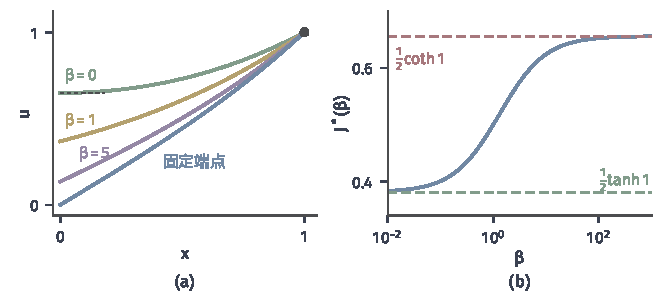
\includegraphics[width=112mm]{figures/05-optimization/08-functional-optimization/matplotlib/func-natural-beta/figure.pdf}
  \caption{从自然边界到固定端点。(a)$u(1)=1$（灰点）时，$\beta=0,1,5$的解和固定端点$u(0)=0$的解（蓝）；绿线在$x=0$处水平，短虚线是水平切线。(b)最优值$J_\beta^\star$随$\beta$从$\frac12\tanh1$上升到$\frac12\coth1$。}
  \label{fig:func-natural-beta}
\end{BookInlineFigure}

\paragraph{端点沿曲线移动}
更一般地，端点的横坐标也可以动。设左端固定在$(a,\alpha)$，右端点要落在给定曲线$y=\psi(x)$上，未知量是函数$u$和右端横坐标$b$。这时积分上限也在变，式~\eqref{eq:func-first-variation-parts}要重新推导。

取一族可行的$(u_t,b_t)$，$t=0$时为$(u,b)$，记$\eta=\partial_tu_t|_{t=0}$，$\tau=\dot{b}_t|_{t=0}$。这里$u$在$b$的右侧邻域内也有定义，$u_t$在其上可导。对积分上限和被积函数分别求导，得到
\[
 \frac{\mathrm{d}}{\mathrm{d}t}J\Big|_{t=0}=F\bigl(b,u(b),u'(b)\bigr)\tau+\int_a^b\bigl(F_s\eta+F_p\eta'\bigr)\,\mathrm{d}x.
\]
约束$u_t(b_t)=\psi(b_t)$对$t$求导，把端点的两种移动联系起来：
\[
 \eta(b)+u'(b)\tau=\psi'(b)\tau.
\]

内部方程仍然成立，因为固定$b$和端点值的扰动仍然允许。代入分部积分，并用$\eta(a)=0$，积分项消失，只剩$F\tau+F_p\eta(b)$。把上式解出的$\eta(b)=(\psi'(b)-u'(b))\tau$代入，由$\tau$可以任意取，得到
\begin{equation}
 F+\bigl(\psi'-u'\bigr)F_p=0\qquad\text{在}\ x=b.
 \label{eq:func-transversality}
\end{equation}
这是\term{横截条件}（transversality condition）。它有别于式~\eqref{eq:func-natural}，因为这里多了由积分上限移动产生的$F\tau$。

用最短曲线检验。对$F=\sqrt{1+p^2}$，式~\eqref{eq:func-transversality}化简为
\[
 \frac{1+\psi'(b)\,u'(b)}{\sqrt{1+u'(b)^2}}=0,
\]
即$\psi'(b)\,u'(b)=-1$。极值曲线是直线，所以结论是：从一点到一条曲线的最短线段垂直于这条曲线。图~\ref{fig:func-transversal}中，曲线是$\psi(x)=2-x$，斜率$-1$，于是$u'=1$。从原点出发的直线$y=x$在$(1,1)$处与之相交，长度$\sqrt2$。

\begin{BookInlineFigure}
  \centering
  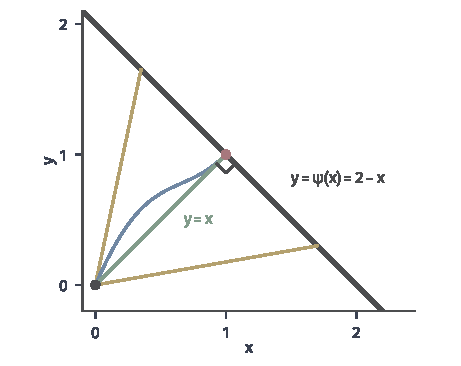
\includegraphics[width=78mm]{figures/05-optimization/08-functional-optimization/matplotlib/func-transversal/figure.pdf}
  \caption{端点沿曲线移动时的最短曲线。深灰粗线是端点可落的直线$y=2-x$，绿色线段是解，在红点$(1,1)$处与之垂直，长度$\sqrt2\approx1.414$。黄色线段端点分别在$x=0.35$和$x=1.7$处，长度分别约为$1.69$和$1.73$；蓝色曲线到同一终点，也比直线长。}
  \label{fig:func-transversal}
\end{BookInlineFigure}

\paragraph{多元区域的边界}
在区域$\Omega$上，分部积分换成散度定理，边界项变成边界积分$\int_{\partial\Omega}(\nabla_{\bm{p}}F\cdot\bm{n})\,\eta\,\mathrm{d}S$，$\bm{n}$是外法向量。边界分成两部分时，固定值的部分上$\eta=0$，放开的部分上，同样的两步推理给出$\nabla_{\bm{p}}F\cdot\bm{n}=0$。对$F=\frac12\lVert\bm{p}\rVert_2^2$，这就是法向导数为零。

各种边界情形可以总结成一张表，共同的来源都是式~\eqref{eq:func-first-variation-parts}的边界项。

\begin{BookInlineTable}
  \centering
  \caption{一维问题右端的三种边界情形，左端符号相反。}
  \label{tab:func-boundary}
  \begin{tabular}{lll}
    \toprule
    端点情形 & 允许的扰动 & 边界条件\\
    \midrule
    固定 $u(b)=\beta$ & $\eta(b)=0$ & $u(b)=\beta$\\
    放开 $u(b)$ & $\eta(b)$ 任意 & $F_p=0$\\
    放开并加代价 $\Phi(u(b))$ & $\eta(b)$ 任意 & $F_p+\Phi'(u(b))=0$\\
    沿曲线 $y=\psi(x)$ 移动 & $\eta(b)=(\psi'-u')\tau$ & $F+(\psi'-u')F_p=0$\\
    \bottomrule
  \end{tabular}
\end{BookInlineTable}

\section{有限维近似}
\label{sec:func-finite}

Euler--Lagrange方程只在少数情形下能解出来。接下来要弄清：怎样把函数问题换成可计算的有限维问题，换完之后算出来的东西离真解有多远？本节开头的向量类比在这里变成计算方法。

\paragraph{主要思想}
可行集$\bm{C}=u_0+\bm{V}$太大，就在其中挑一个有限维的小块。取线性无关的\term{试探函数}（trial function）$\phi_1,\ldots,\phi_r\in\bm{V}$，令$\bm{V}_n$是它们张成的子空间，只在
\begin{equation}
 \bm{C}_n=u_0+\bm{V}_n
 \label{eq:func-trial}
\end{equation}
中比较候选。$\bm{V}_n$称为\term{试探空间}（trial space），$n$表示近似的精细程度。候选由系数向量$\bm{c}\in\mathbb{R}^r$决定，目标泛函变成普通的多元函数$f(\bm{c})=J(u_0+\sum_ic_i\phi_i)$。在试探空间上直接最小化目标的做法称为\term{Ritz方法}（Ritz method）。

这样得到的问题前面各章都能解，$\bm{C}_n\subseteq\bm{C}$也保证了离散最优值不低于$J^\star$。对二次目标，步骤可以完全写出来。设$J(u)=\frac12a(u,u)-\xi(u)$，$a$是对称双线性形式，$\xi$是线性泛函。代入并按$\bm{c}$整理，得到
\begin{equation}
 f(\bm{c})=J(u_0)+\frac12\bm{c}^\top\bm{A}\bm{c}-\bm{b}^\top\bm{c},
 \label{eq:func-ritz-quadratic}
\end{equation}
其中
\begin{equation}
 \bm{A}_{i,j}=a(\phi_i,\phi_j),\qquad b_i=\xi(\phi_i)-a(u_0,\phi_i).
 \label{eq:func-ritz-matrix}
\end{equation}
若$a$在$\bm{V}$上正定，$\bm{A}$对称正定，令梯度为零得到唯一的解
\begin{equation}
 \bm{c}=\bm{A}^{-1}\bm{b},\qquad \min f=J(u_0)-\frac12\bm{b}^\top\bm{c}.
 \label{eq:func-ritz-solution}
\end{equation}

最简单的例子只用一个试探函数。对$E$取$u_0=x$，$\phi_1=x(1-x)$，由式~\eqref{eq:func-phi-example}，$A_{1,1}=11/30$，$b_1=-1/12$。于是$c_1=-5/22$，这正是图~\ref{fig:func-direction-family}(b)的最小点。由式~\eqref{eq:func-ritz-solution}，目标值是
\[
 \frac23-\frac{5}{528}=\frac{347}{528}\approx0.65720.
\]
而$E^\star\approx0.65652$。一个参数就把目标差从$0.0101$降到$0.0007$。

\paragraph{计算过程}
下面用分段线性的试探函数，继续计算目标$E$，$u(0)=0$，$u(1)=1$。这时$a(v,w)=\int_0^1(v'w'+vw)\,\mathrm{d}x$，$\xi=0$。

\needspace{6\baselineskip}
\paragraph{变量}
\begin{itemize}
 \item 段数$n$，步长$\Delta=1/n$，结点$x_i=i\Delta$。例中$n=3$，$\Delta=1/3$。
 \item 帐篷函数$\phi_i$：在结点$x_i$处为$1$，其他结点为零，其间线性。自由系数$\bm{c}\in\mathbb{R}^{r}$，$r=n-1$，$c_i$就是结点$x_i$的高度。
 \item 三对角矩阵$\bm{A}\in\mathbb{R}^{r\times r}$和向量$\bm{b}\in\mathbb{R}^{r}$，由式~\eqref{eq:func-ritz-matrix}定义。
\end{itemize}

\paragraph{初始化}
取$u_0$满足边界条件。例中取右端的半个帐篷$u_0=\phi_3$，它在$x=1$处为$1$，在其余结点为零。图~\ref{fig:func-ritz-hats}(a)画了这三个函数。

\paragraph{组装与求解}
\begin{enumerate}
 \item 计算相邻帐篷的内积。每个帐篷的导数是$\pm1/\Delta$，直接积分得到
 \begin{equation}
  a(\phi_i,\phi_i)=\frac{2}{\Delta}+\frac{2\Delta}{3},\qquad a(\phi_i,\phi_{i+1})=-\frac1\Delta+\frac\Delta6,
  \label{eq:func-hat-matrix}
 \end{equation}
 不相邻的帐篷内积为零，边界上的半个帐篷$a(\phi_n,\phi_n)=\frac1\Delta+\frac\Delta3$。例中
 \[
  a(\phi_1,\phi_1)=a(\phi_2,\phi_2)=\frac{56}{9},\qquad a(\phi_1,\phi_2)=-\frac{53}{18},\qquad a(\phi_3,\phi_3)=\frac{28}{9}.
 \]
 
 \item 由式~\eqref{eq:func-ritz-matrix}组装。例中$\phi_3$只和$\phi_2$相邻，所以
 \[
  \bm{A}=\begin{bmatrix}56/9&-53/18\\-53/18&56/9\end{bmatrix},\qquad\bm{b}=\begin{bmatrix}0\\53/18\end{bmatrix}.
 \]
 
 \item 解线性方程组$\bm{A}\bm{c}=\bm{b}$。例中两边乘以$18$，得到
 \[
  112c_1-53c_2=0,\qquad-53c_1+112c_2=53.
 \]
 由第一式，$c_1=53c_2/112$。代入第二式，解得
 \[
  c_1=\frac{2809}{9735}\approx0.28855,\qquad c_2=\frac{5936}{9735}\approx0.60976.
 \]
 
 \item 由式~\eqref{eq:func-ritz-solution}计算目标值。例中$J(u_0)=\frac12a(\phi_3,\phi_3)=\frac{14}{9}$，于是
 \[
  E_3=\frac{14}{9}-\frac12\cdot\frac{53}{18}\cdot\frac{5936}{9735}\approx0.65786.
 \]
\end{enumerate}

最终得到结点高度$(0,\,0.28855,\,0.60976,\,1)$的折线。真解在相同结点的值是$0.28892$和$0.61024$，$E^\star\approx0.65652$，见图~\ref{fig:func-ritz-hats}(b)。$n$增大时，$\bm{A}$是三对角矩阵，每次求解的代价正比于$n$。

\begin{BookInlineFigure}
  \centering
  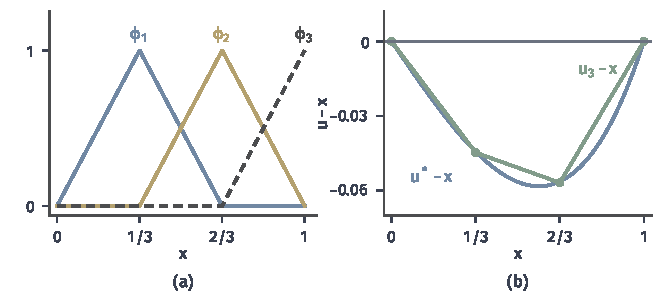
\includegraphics[width=112mm]{figures/05-optimization/08-functional-optimization/matplotlib/func-ritz-hats/figure.pdf}
  \caption{$n=3$的Ritz方法。(a)帐篷函数$\phi_1,\phi_2$是自由方向，虚线$\phi_3$用来满足$u(1)=1$。(b)为了看清差别，画的是$u-x$：蓝色为真解，绿色折线为Ritz解，结点值接近真解的结点值。}
  \label{fig:func-ritz-hats}
\end{BookInlineFigure}

\paragraph{自然边界条件不必写进试探空间}
第~\ref{sec:func-free-boundary}小节的问题中左端自由。Ritz方法的处理非常简单：不约束$x=0$处的结点，把$\phi_0$加入试探函数。条件$u'(0)=0$不写进任何地方。

$n=1$时只有一个未知数$u(0)$，$a(\phi_0,\phi_0)=4/3$，$a(\phi_0,\phi_1)=-5/6$，解得$u(0)=5/8$。这条直线的斜率不为零，自然条件并不精确成立，它要靠加密来逼近。图~\ref{fig:func-ritz-natural}中，$n=3$时左端第一段的斜率降到$0.110$，$u(0)=0.6457$，真解是$1/\cosh1\approx0.6481$。目标值$0.4063$、$0.3835$也逐步接近$E^\star\approx0.3808$。

\begin{BookInlineFigure}
  \centering
  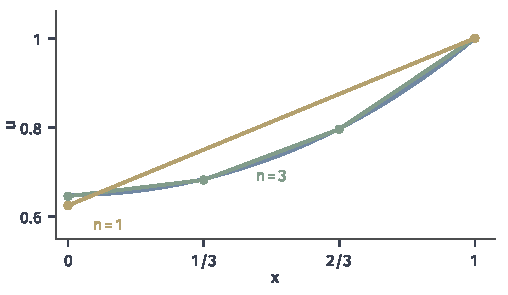
\includegraphics[width=86mm]{figures/05-optimization/08-functional-optimization/matplotlib/func-ritz-natural/figure.pdf}
  \caption{左端自由时的Ritz解。蓝色是真解$\cosh x/\cosh1$，黄色是$n=1$，绿色是$n=3$。试探空间没有写入$u'(0)=0$，第一段的斜率随加密而趋于零。}
  \label{fig:func-ritz-natural}
\end{BookInlineFigure}

先离散再优化，和先写出方程再离散，是两条路线。对$E$，后者用差分代替二阶导数，内部结点的方程是$\frac1\Delta(-u_{i-1}+2u_i-u_{i+1})+\Delta u_i=0$，而Ritz方法的$\Delta u_i$项换成了$\frac\Delta6(u_{i-1}+4u_i+u_{i+1})$。$n=3$时，差分解的结点值是$0.28929$和$0.61071$，精度相当。差别在于结构：Ritz方法的矩阵自动对称，目标值从上方逼近$E^\star$，自然边界条件自动处理；差分方法要为边界单独设计格式。

\paragraph{三种误差}
算出的结果与真解的距离由几件不同的事情决定，必须分开。下面逐一说明，它们的区别列在表~\ref{tab:func-errors}中。

第一件事是固定函数能否被逼近：给定一个$v\in\bm{C}$，$\bm{C}_n$中有没有函数$v_n$，使$J(v_n)\to J(v)$。这是试探空间和目标的性质，与优化无关。例如$v=x+\frac14\sin2\pi x$，取它的线性插值$v_n$，$\lvert E(v_n)-E(v)\rvert$按$n^{-2}$衰减，见图~\ref{fig:func-three-errors}(a)的黄线。

第二件事是离散极小者$u_n$是否收敛到真解，这要求$J(u_n)\to J^\star$，还要求$u_n$本身收敛。它比第一件事多要求目标有存在性论证那样的结构。第三件事是数值求解误差：实际算出的$\tilde{u}_n$与精确的离散极小者$u_n$之间的差。

\begin{BookInlineTable}
  \centering
  \caption{三种误差。}
  \label{tab:func-errors}
  \begin{tabular}{lll}
    \toprule
    误差 & 比较的对象 & 决定因素\\
    \midrule
    固定函数逼近 & $J(v_n)$ 与 $J(v)$ & 试探空间、$J$ 的连续性\\
    离散极小者收敛 & $u_n$ 与 $u^\star$ & 上一项及存在性结构\\
    数值求解 & $\tilde{u}_n$ 与 $u_n$ & 算法与迭代步数\\
    \bottomrule
  \end{tabular}
\end{BookInlineTable}

\paragraph{二次目标：Ritz解是能量范数下的最佳逼近}
对二次目标，第二件事可以精确回答。目标值的差恰好是一个距离的平方，下面的定理把“目标最小”变成“离真解最近”。

\begin{theorem}[Ritz方法的最佳逼近性质]
\label{thm:func-cea}
设$\bm{V}$是Hilbert空间，$a$是$\bm{V}$上的对称双线性形式，存在$0<\mu\leq L$，使
\begin{equation}
 \mu\lVert\eta\rVert^2\leq a(\eta,\eta)\leq L\lVert\eta\rVert^2\qquad(\eta\in\bm{V}),
 \label{eq:func-a-bounds}
\end{equation}
并且$J(u)=\frac12a(u,u)-\xi(u)$在$\bm{C}=u_0+\bm{V}$上有极小点$u^\star$。则对$v\in\bm{C}$，
\begin{equation}
 J(v)-J(u^\star)=\frac12a(v-u^\star,v-u^\star).
 \label{eq:func-energy-identity}
\end{equation}
若$u_n$是$J$在$\bm{C}_n=u_0+\bm{V}_n$上的极小点，则
\begin{equation}
 a(u_n-u^\star,\,u_n-u^\star)=\min_{v\in\bm{C}_n}a(v-u^\star,\,v-u^\star),
 \label{eq:func-cea}
\end{equation}
并且
\begin{equation}
 \lVert u_n-u^\star\rVert\leq\sqrt{\frac{L}{\mu}}\,\min_{v\in\bm{C}_n}\lVert v-u^\star\rVert.
 \label{eq:func-cea-norm}
\end{equation}
\end{theorem}

\begin{proof}
令$\eta=v-u^\star\in\bm{V}$，把$J(u^\star+\eta)$按$\eta$展开：
\[
 J(u^\star+\eta)-J(u^\star)=DJ(u^\star)[\eta]+\frac12a(\eta,\eta).
\]
由式~\eqref{eq:func-stationary}，一次项为零，得到式~\eqref{eq:func-energy-identity}。

$u_n$使左端在$\bm{C}_n$上最小，也就使$a(v-u^\star,v-u^\star)$最小，这就是式~\eqref{eq:func-cea}。对任意$v\in\bm{C}_n$，由$a$的两个界，
\[
 \mu\lVert u_n-u^\star\rVert^2\leq a(u_n-u^\star,u_n-u^\star)\leq a(v-u^\star,v-u^\star)\leq L\lVert v-u^\star\rVert^2.
\]
开方并对$v$取最小，得到式~\eqref{eq:func-cea-norm}。
\end{proof}

式~\eqref{eq:func-energy-identity}的直观是：能量地形是一只以$u^\star$为底的碗，比较目标值就是比较到碗底的距离。式~\eqref{eq:func-cea}说明，Ritz方法不需要事先知道$u^\star$，却自动选出了$u^\star$在试探空间中的最佳逼近。在式~\eqref{eq:func-energy}的例子上，$a$就是$H^1$内积，$\mu=L=1$，Ritz解是$u^\star$在$H^1$范数下的正交投影。

这也把收敛速度转化成逼近问题。线性元逼近$H^1$函数的误差按$\Delta$衰减，目标差是距离的平方，按$\Delta^2$衰减。图~\ref{fig:func-three-errors}(a)的绿线实测：$n=16,32,64$时目标差为$4.79\times10^{-5}$、$1.20\times10^{-5}$、$3.00\times10^{-6}$，每次缩小到四分之一。

\begin{BookInlineFigure}
  \centering
  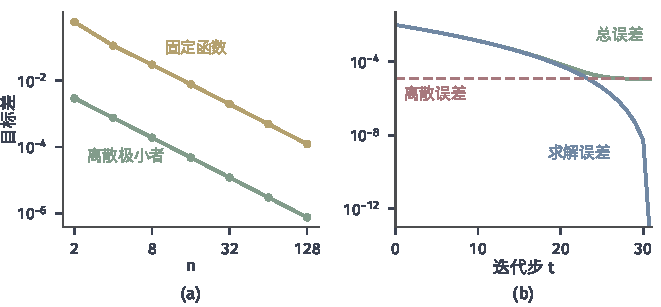
\includegraphics[width=112mm]{figures/05-optimization/08-functional-optimization/matplotlib/func-three-errors/figure.pdf}
  \caption{目标$E$的三种误差。(a)黄色是固定函数$x+\frac14\sin2\pi x$的线性插值的能量误差，绿色是Ritz解的目标差$E(u_n)-E^\star$，两者都按$n^{-2}$衰减。(b)$n=32$时用共轭梯度法从$u=x$出发：蓝色是求解误差$E(\tilde{u}_n)-E(u_n)$，绿色是总误差$E(\tilde{u}_n)-E^\star$，红色虚线是离散误差$1.20\times10^{-5}$。}
  \label{fig:func-three-errors}
\end{BookInlineFigure}

\paragraph{一般目标的收敛}
对非二次的目标，能保证的结论要弱一些，证明正好回用第~\ref{sec:func-existence}节的论证。这里用$\tilde{u}_n$同时把求解误差包括进来。

\begin{theorem}[Ritz方法的收敛]
\label{thm:func-ritz-convergence}
设$X$、$\bm{C}$和$J$满足定理~\ref{thm:func-direct-method}中反射、弱序列闭和弱序列下半连续的条件，$J$的每个下水平集都有界，$J$在$\bm{C}$上按范数连续且处处有限，$\bm{C}_n\subseteq\bm{C}$非空。设对每个$v\in\bm{C}$，存在$v_n\in\bm{C}_n$使$v_n\to v$。若$\tilde{u}_n\in\bm{C}_n$满足
\begin{equation}
 J(\tilde{u}_n)\leq\inf_{\bm{C}_n}J+\varepsilon_n,\qquad\varepsilon_n\to0,
 \label{eq:func-approx-minimizer}
\end{equation}
则$J(\tilde{u}_n)\to J^\star$，$\tilde{u}_n$有弱收敛子列，且每个弱收敛子列的极限都是最优解。
\end{theorem}

\begin{proof}
任取$\varepsilon>0$和$v\in\bm{C}$，使$J(v)\leq J^\star+\varepsilon$。取$v_n\to v$，由连续性$J(v_n)\to J(v)$。由式~\eqref{eq:func-approx-minimizer}，
\[
 J^\star\leq J(\tilde{u}_n)\leq J(v_n)+\varepsilon_n.
\]
令$n\to\infty$，再令$\varepsilon\to0$，得到$J(\tilde{u}_n)\to J^\star$。所以$\tilde{u}_n$是极小化序列。

下水平集有界，所以序列有界，由反射性有弱收敛子列。设某子列弱收敛到$u$，$\bm{C}$弱序列闭给出$u\in\bm{C}$，弱序列下半连续给出$J(u)\leq J^\star$，所以$u$是最优解。
\end{proof}

定理说明Ritz方法产生的是一个极小化序列，第~\ref{sec:func-existence}节的三关同时决定了它的命运。若$J$还满足$J(v)-J^\star\geq\frac\mu2\lVert v-u^\star\rVert^2$，例如$J$是$\mu$-强凸的，则目标收敛蕴含范数收敛。

\paragraph{各条件的作用}
条件去掉，结论就会失败。连续性保证“固定函数的能量能被逼近”。若$J$不连续，$\bm{C}_n$稠密也不够：存在目标使得Lipschitz函数上的下确界严格大于$W^{1,1}$上的下确界，这称为Lavrentiev现象，经典例子是Manià给出的。这时分段线性的试探函数永远达不到真正的下确界，证明较长，读者可查阅变分法的专著。

弱序列下半连续保证极限真的最优。对目标~\eqref{eq:func-bolza}，取$n$为偶数的线性元，结点值交替取$0,\Delta,0,\Delta,\ldots$的折线就是图~\ref{fig:func-bolza-zigzag}的锯齿，所以
\[
 0<\min_{\bm{C}_n}J\leq\frac{\Delta^2}{3}.
\]
每个离散问题都有解，最优值也收敛到$J^\star=0$，离散解的振幅趋于零，一致趋于$u=0$。但$J(0)=1$，这个极限根本不是解，原问题也没有解。计算机算出的“收敛”数字，不能代替第~\ref{sec:func-existence}节的存在性论证。

\paragraph{数值求解误差}
对二次目标，由式~\eqref{eq:func-energy-identity}（把它用在$\bm{C}_n$上，$u_n$代替$u^\star$），两种误差恰好相加：
\begin{equation}
 J(\tilde{u}_n)-J^\star=\frac12a(\tilde{u}_n-u_n,\tilde{u}_n-u_n)+\bigl(J(u_n)-J^\star\bigr).
 \label{eq:func-error-split}
\end{equation}
第一项是求解误差，第二项是离散误差。图~\ref{fig:func-three-errors}(b)中，共轭梯度法的总误差下降到约$25$步后就贴住了离散误差，再多的迭代只减少第一项。所以迭代的停止精度应该与离散误差相称，把线性方程组解到机器精度是浪费。

矩阵$\bm{A}$的条件数按$n^2$增长，这是第~\ref{sec:func-hilbert-gradient}小节讲过的现象。用刚度矩阵作预条件，相当于换成$H^1$型内积，迭代次数就基本不随网格变化。

\paragraph{非二次目标}
非二次目标的离散问题用前面各章的方法求解，第~\ref{chap:second-order-methods}章的牛顿法尤其合适。考虑
\[
 J(u)=\int_0^1\Bigl(\frac12u'(x)^2+\frac14u(x)^4\Bigr)\,\mathrm{d}x,\qquad u(0)=0,\ u(1)=1.
\]
它满足定理~\ref{thm:func-tonelli}，又是严格凸的，解存在且唯一。取$u=x+c\,x(1-x)$，用Beta积分把$x^4(1+c(1-x))^4$逐项积分，得到一元多项式
\[
 f(c)=\frac{11}{20}+\frac{c}{30}+\frac{19}{105}c^2+\frac{c^3}{280}+\frac{c^4}{2520}.
\]

从$c^{(0)}=0$出发用牛顿法。第一步，$f'(0)=\frac1{30}$，$f''(0)=\frac{38}{105}$，于是
\[
 c^{(1)}=-\frac{7}{76}\approx-0.09211.
\]
第二步，$f'(c^{(1)})\approx8.97\times10^{-5}$，$f''(c^{(1)})\approx0.35997$，于是
\[
 c^{(2)}\approx-0.09235.
\]
此时$f\approx0.548462$，比$f(0)=0.55$低，再迭代目标值几乎不变。

对线性元离散的完整问题，牛顿法的Hessian是三对角的，每步代价正比于$n$。图~\ref{fig:func-newton-mesh}中，$n=8,32,128$的三条残差曲线几乎重合，都在$3$步内到达机器精度，这称为网格无关性。这个性质表明，牛顿法的步数是函数问题本身的性质，而不是某个离散向量问题的性质。

\begin{BookInlineFigure}
  \centering
  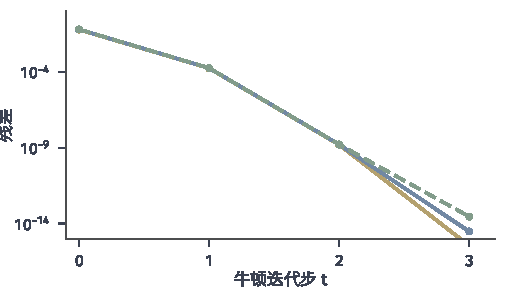
\includegraphics[width=86mm]{figures/05-optimization/08-functional-optimization/matplotlib/func-newton-mesh/figure.pdf}
  \caption{牛顿法的网格无关性。目标$\int_0^1(\frac12u'^2+\frac14u^4)\,\mathrm{d}x$，从$u=x$出发，线性元、梯形求积。纵轴是在$\bm{K}^{-1}$范数下度量的梯度残差，$\bm{K}$是刚度矩阵，它对应函数空间的对偶范数。黄、蓝、绿虚线分别是$n=8,32,128$，三条线几乎重合。}
  \label{fig:func-newton-mesh}
\end{BookInlineFigure}

\section{本章小结}
\label{sec:func-summary}

章首的问题是：未知量是一整条曲线时，怎样找最好的那一条。函数可以看成很长的向量，泛函梯度对应向量梯度，这个类比决定了本章的工作顺序：先证存在，再用微分判别，最后离散计算。

\paragraph{三件工具各负责什么}
弱极限与下半连续性负责证明存在。无限维的闭球不紧，只能取弱收敛子列，于是可行集要弱序列闭，目标要弱序列下半连续。凸性让这两个条件可以检查，定理~\ref{thm:func-direct-method}把它们串起来。第~\ref{sec:func-existence}节的四个反例分别对应缺少强制性、反射性、弱闭性和对导数的凸性。写出驻定方程不能代替这一步。

微分与变分负责判别候选。方向导数、Gâteaux微分和Fréchet微分逐层加强，差别在于余项是否对方向一致，并且依赖范数。微分经Riesz表示才成为梯度，梯度依赖内积，也可能不存在。一阶条件和凸性充分性与有限维一致，二阶充分性需要统一的曲率下界，乘子法则在有限个约束下成立，无穷约束下要重新检查拓扑。

试探空间负责把函数问题转成有限维计算。Ritz方法在二次目标上给出能量范数下的最佳逼近。固定函数的能量逼近、离散极小者的收敛、数值求解的误差是三件不同的事。

\paragraph{积分目标的结论}
积分泛函的一阶变分经分部积分，分成内部的Euler--Lagrange方程和一个边界项。内部方程来自两端固定的扰动，边界条件来自放开的扰动：端点值自由给出$F_p=0$，端点沿曲线移动给出横截条件。这些方程都是必要条件，极小性要靠凸性或二阶条件来确认。

\begin{BookInlineTable}
  \centering
  \caption{本章的问题、工具与条件。}
  \label{tab:func-summary}
  \begin{tabular}{lll}
    \toprule
    问题 & 工具 & 关键条件\\
    \midrule
    解是否存在 & 直接法 & 反射、弱闭、弱下半连续\\
    候选怎样判别 & 微分与变分 & 所选范数下可微、凸性\\
    方程与边界 & 分部积分 & 正则性、允许的扰动\\
    怎样计算 & Ritz方法 & 稠密、连续、求解精度\\
    \bottomrule
  \end{tabular}
\end{BookInlineTable}

\paragraph{边界}
本章只建立优化问题本身的存在性、判别和近似。Euler--Lagrange方程解的存在性、正则性和具体边值问题的理论属于微分方程部分；以概率分布为未知量的变分问题由\BookChapterRef{chap:probability-distribution-optimization}{卷七第12章“概率分布的优化与逼近”}研究。离散之后的有限维问题，用本卷前面各部分的方法求解。

